\documentclass[11pt]{article}
\usepackage{amsmath,amssymb}
\DeclareMathOperator{\E}{\mathbb{E}} % For the expectation style E
\usepackage{graphicx}
\usepackage{tabularx}
\usepackage[a4paper, total={6.5in, 9.5in}]{geometry} % Set margin size.
%\usepackage{subfigure}
\usepackage{subcaption}
\usepackage{amsfonts}
\usepackage{bm}

\usepackage{setspace}
%\onehalfspacing
%\doublespacing

\begin{document}

\begin{titlepage}
                % \newgeometry{top=25mm,bottom=25mm,left=38mm,right=32mm}
                \setlength{\parindent}{0pt}
                \setlength{\parskip}{0pt}
                % \fontfamily{phv}\selectfont

                {
                                \Large
                                \raggedright
                                Imperial College London\\[17pt]
                                Department of Electrical and Electronic Engineering\\[17pt]
                                Final Year Project Report 2018\\[17pt]
 
                }

                \rule{\columnwidth}{3pt}
                \vfill
                \centering
                  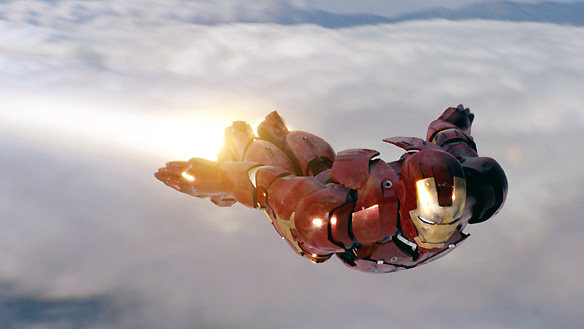
\includegraphics[width=\columnwidth]{cover.jpg}
                \vfill
                \setlength{\tabcolsep}{0pt}

                \begin{tabular}{p{40mm}p{\dimexpr\columnwidth-40mm}}
                                Project Title: & \textbf{Investigating practical ion propulsion engines} \\[12pt]
                                Student: & \textbf{Agni Iyer} \\[12pt]
                                CID: & \textbf{00985557} \\[12pt]
                                Course: & \textbf{EEE3} \\[12pt]
                                Project Supervisor: & \textbf{Dr Stepan Lucyszyn} \\[12pt]
                \end{tabular}
\end{titlepage}


\tableofcontents
\pagebreak

\section{Abstract}

Electric propulsion technology generates thrust without any fuel, emissions, moving parts or heat signature, and is primarily used in deep space exploration and attitude adjustment for satellites. Given the projected growth in communication satellites that will be in orbit to provide Internet access to a growing global population, it is a sector that is poised for substantial growth. This project aims to investigate whether the principles of ion propulsion engines, and more specifically electrohydrodynamic (EHD) propulsion, can be used as a practical source of generating thrust on Earth. The project begins with a brief history of the technology and an overview and comparison of the various types of electric thrusters. Hall thrusters and ion thrusters are the most widely used, so their operating principles have been explained in detail. This is followed by a theoretical overview of corona discharge and their application in ion propelled aircrafts known as ionocrafts. The design and construction process of a stationary EHD thruster and an ionocraft are outlined in detail, followed by extensive testing to verify the effect of varying input power, duty cycle, and frequency.  

\pagebreak

\section{Acknowledgements}

This project would not have been successful without the help of a few key individuals. I would like to thank Dr Stepan Lucyszyn for proposing the project and for taking the time to supervise its execution, Mr Victor Boddy for his extensive guidance during construction and testing of the prototypes, Mr Phil Jones for helping me fabricate the thruster in the mechanical workshop, Dr Aaron Knoll from the Department of Aeronautical Engineering for his insight into electric propulsion technologies and feedback on the project, and Mr Hisham Maarki for helping me procure all the necessary components required in a timely manner. Lastly, and most importantly, I would like to thank my family for their constant support and encouragement throughout the project.

\pagebreak

\section{Introduction}

Electric propulsion (EP) technology generates thrust by using electricity to increase the propellant exhaust velocity. Spacecraft powered by typical EP systems may eject propellant at up to 20 times the speed of conventional chemical systems, delivering a much higher specific impulse (Isp), or the amount of thrust obtained for the weight of fuel burned \cite{nasa}. They also have 10 times the mileage (miles per gallon of propellant) of chemical rockets. For space applications, the reduced propellant mass can enable the use of a smaller aircraft, and thus lower cost, to deliver an object into orbit or deep space.\\

While the maximum velocity that can be achieved by a chemical rocket is about 5 kilometers per second, a Hall thruster could get a craft up to 40 kilometers per second \cite{space}. However, EP systems produce very low thrust, so they will take a long time to reach these velocities. Since the thruster is silent, has no moving parts, no emissions, and no heat signature (making it invisible to infrared detectors), there are a number of potential military and security applications.\\

The main aim of this project is to build and investigate prototypes of ion thrusters, a leading type of electric propulsion technology, and ionocrafts, a device that uses an electrohydrodynamic phenomenon to produce thrust in air, to understand the factors that affect their performance and explore possible avenues for improving thrust output and large scale applications.


%\pagebreak
\section{Background}

\subsection{A Brief History}

The idea of \textbf{electric propulsion} was first put forward very briefly by Robert Goddard in 1906 and independently by Tsiolkovskiy in Russia in 1911. The first systematic analysis of electric propulsion was made in 1964 by Ernst Stuhlinger in his book \textit{Ion Propulsion for Space Flight} and the physics of ion thrusters was described comprehensively by Robert Jahn in 1968. In the 1960s, the National Aeronautics and Space Administration (NASA) in the United States and several institutes in Russia established electric propulsion research programs for satellite station keeping and deep space applications. The first experimental ion thrusters were launched into orbit in the early 1960s by the US and Russia, and experimental test flights of ion thrusters continued from that time into the 1980s.\\

The principle of \textbf{ionic wind propulsion} with corona-generated charged particles has been known from the earliest days of the discovery of electricity, with references dating back to 1709 in a book titled \textit{Physico-Mechanical Experiments on Various Subjects} by Francis Hauksbee. Major Alexander Prokofieff de Seversky pioneered its application to propulsion systems by developing the basic physics and prototype designs in 1960. In 1964, he coined the term \textit{Ionocraft} in his U.S. Patent US3130945A for the technology.\\

\begin{figure}[h!]
\centering
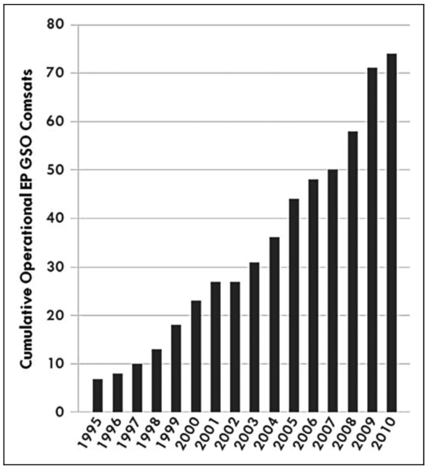
\includegraphics[width= 0.4\textwidth]{comsats}
\caption{\label{fig:comsats} Diagram showing the increasing number of satellites using EP for station-keeping \cite{comstat}}
\end{figure}

Over the past few decades, electric propulsion use has grown steadily worldwide as an alternative to chemical thrusters to reduce the propellant mass for station-keeping and orbit insertion of geosynchronous communication satellites. The US and Russia have each flown over a 100 ion thrusters in communication satellites, and there are a number of planned launches for communication satellites and space missions that will continue to take advantage of the reliability and cost effectiveness of this technology.

\pagebreak
\subsection{Types of electric thrusters}

Electric propulsion technologies can be divided into 3 categories based on the method of acceleration used to produce the thrust: electro-thermal, electrostatic, and electromagnetic. Common thruster types are \cite{goebel}:

\begin{enumerate}
\item \textbf{Resistojet}: An electro-thermal device in which propellant is heated by passing through a resistively heated chamber or element before passing through a downstream nozzle. The increase in exhaust velocity is due to thermal heating of the propellant. This limits the Isp to low levels (less than 500s).

\item \textbf{Arcjet}: Electrothermal thruster that heats the propellant by passing it though a high current arc in line with the nozzle feed system. Although there is an electric discharge in the propellant path, plasma effects are negligible in the exhaust velocity since the propellant is weakly ionized. The Isp is limited by the thermal heating to less than about 700s for easily stored propellants.

\item \textbf{Ion Thruster}: Ion thrusters use a variety of plasma generation methods to ionize a large portion of the propellant. Biased grids then extract ions from the plasma and accelerate them to high velocity at voltages up to and exceeding 10 kV. These thrusters have the \textbf{highest efficiency} (from 60\% to  more than 80\%) and \textbf{very high Isp} (from 2000s to over 10,000s) compared to other thruster types.

\item \textbf{Hall Thruster}: An electrostatic thruster that uses a cross-field discharge described by the Hall effect to generate the plasma. An electric field established perpendicular to an applied magnetic field  accelerates ions to high exhaust velocities, while the transverse magnetic field inhibits electron motion that would tend to short out the electric field. Efficiency and Isp are less than that achievable by ion thrusters, but the \textbf{thrust at a given power is higher}, the device is much \textbf{simpler} and requires \textbf{fewer power supplies} to operate.

\item \textbf{Electrospray/Field Emission Electric Propulsion Thruster}: These are two types of electrostatic EP devices that generate very low thrust (less than 1 mN). Electrospray thrusters extract ions or charged droplets from conductive liquids fed through small needles and accelerate them electrostatically with biased aligned apertures to high energy. Field emission electric propulsion (FEEP) thrusters wick or transport liquid metals (typically indium or cesium) along needles, extracting ions from the sharp tip by field emission processes. Due to their very low thrust, these devices are used for precision control of spacecraft position or attitude in space.

\item \textbf{Pulsed Plasma Thruster}: An electromagnetic thruster that utilizes a pulsed discharge to ionize a fraction of a solid propellant ablated into a plasma arc. Electromagnetic effects in the pulse are then used to accelerate the ions to high exit velocity. The pulse repetition rate determines the thrust level.

\item \textbf{Magnetoplasmadynamic (MPD) thruster}: These are electromagnetic devices that use a very high current arc to ionize a significant fraction of the propellant. Electromagnetic forces (Lorentz forces) in the plasma discharge are then used to accelerate the charged propellant. Since both the current and the magnetic field are usually generated by the plasma discharge, MPD thrusters tend to operate at very high powers in order to generate sufficient force for high Isp operation.  This generates higher thrust compared to the other thruster types.

\end{enumerate}


%\pagebreak
The following table summarizes the operating parameters of the main thruster types:

\begin{table}[h!]
\centering
\resizebox{\textwidth}{!} % Fit table to page width
{
\begin{tabular}{|c|c|c|c|c|}
\hline
\textbf{Thruster}         & \textbf{Specific Impulse (s)} & \textbf{Input Power (kW)} & \textbf{Efficiency Range (\%)} & \textbf{Propellant} \\ \hline
Cold gas                  & 50 - 75                       & -                         & -                              & Various             \\ \hline
Chemical (monopropellant) & 150 - 225                     & -                         & -                              & $N_2H_4$ , $H_2O_2$ \\ \hline
Chemical (bipropellant)   & 300 - 450                     & -                         & -                              & Various             \\ \hline
Resistojet                & 300                           & 0.5 - 1                   & 65 - 90                        & $N_2H_4$ monoprop   \\ \hline
Arcjet                    & 500 - 600                     & 0.9 - 2.2                 & 25 - 45                        & $N_2H_4$ monoprop   \\ \hline
Ion Thruster              & 2500 - 3600                   & 0.4 - 4.3                 & 40 - 80                        & Xenon               \\ \hline
Hall Thruster             & 1500 - 2000                   & 1.5 - 4.5                 & 35 - 60                        & Xenon               \\ \hline
PPTs                      & 850 - 1200                    & \textless 0.2             & 7 - 13                         & Teflon              \\ \hline
\end{tabular}
}
\caption{Typical operating parameters for thrusters \cite{goebel}}
\label{}
\end{table}


\subsection{Operating principle of an Ion thruster}

An ion thruster ionizes propellant by adding or removing electrons to produce ions. This is usually carried out by electron bombardment: a high-energy electron (negative charge) collides with a propellant atom (neutral charge), releasing electrons from the propellant atom and resulting in a positively charged ion. The gas produced consists of an equal number of positive ions and negative electrons so that there is no overall electric charge. This is called a plasma.\\

Plasma has some of the properties of a gas, but it is affected by electric and magnetic fields. Common examples are lightning and the substance inside fluorescent light bulbs. The most common propellant used in ion propulsion is xenon. It is easily ionized and has a high atomic mass, thus generating a desirable level of thrust when ions are accelerated. It also is inert and has a high storage density which makes it suitable for storage aboard a spacecraft.\\

\begin{figure}[h!]
\centering
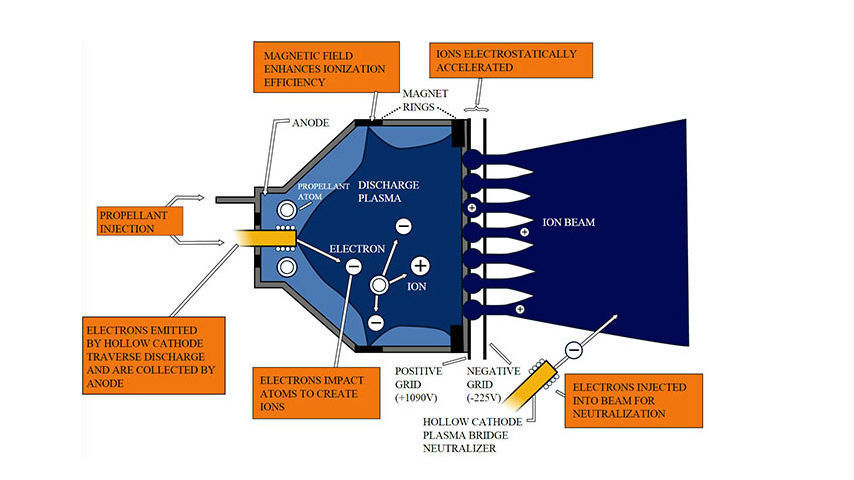
\includegraphics[width= \textwidth]{ion_thrust}
\caption{\label{fig:ion_thrust} Cross section of a typical gridded ion thruster \cite{ionthruster}}
\end{figure}

In most ion thrusters, electrons are generated with the discharge hollow cathode by a process called thermionic emission. Electrons produced by the cathode are attracted to the discharge chamber walls, which are charged to a high positive potential by the voltage applied by the thruster’s power supply. Neutral propellant is injected into the discharge chamber, where the electrons bombard the propellant to produce positively charged ions and release more electrons. Strong magnets prevent electrons from freely reaching the discharge channel walls. This lengthens the time that electrons reside in the discharge chamber and increases the probability of an ionizing event.\\

The positively charged ions migrate toward grids that contain thousands of very precisely aligned holes (apertures) at the aft end of the ion thruster. The first grid is the positively charged electrode (screen grid). A very high positive voltage is applied to the screen grid, but it is configured to force the discharge plasma to reside at a high voltage. As ions pass between the grids, they are accelerated toward a negatively charged electrode (the accelerator grid) to very high speeds (up to 90,000 mph).\\

The discharge cathode and anode represent the plasma generator in Figure \ref{fig:ion_thrust}, and ions from this region flow to the grids and are accelerated to form the thrust beam. The plasma generator is at high positive voltage compared to the spacecraft or space plasma and, therefore, is enclosed in a “plasma screen” biased near the spacecraft potential to eliminate electron collection from the space plasma to the positively biased surfaces. The neutralizer cathode is positioned outside the thruster and provides electrons at the same rate as the ions to avoid charge imbalance with the spacecraft.\\

Ion thrusters that use alternative plasma generators, such as microwave or radio frequency (RF) plasma generators, have the same basic geometry with the plasma generator enclosed in a plasma screen and coupled to a gridded ion accelerator with a neutralizer cathode. The performance of the thruster depends on the plasma generator efficiency and the ion accelerator design.

\pagebreak
\subsection{Operating principle of a Hall Thruster}

A Hall thruster consists of three main parts: the cathode, the discharge region, and the magnetic field generator. Figure \ref{fig:hall_thruster} shows a schematic cross section of a typical Hall thruster. In this example, a cylindrical insulating channel encloses the discharge region. Magnetic coils (not shown) induce a radial magnetic field between the center pole piece and the flux return path at the outside edge. The cathode of the discharge is an external hollow cathode, and the anode is a ring located at the base of the cylindrical slot shown.\\

\begin{figure}[h!]
\centering
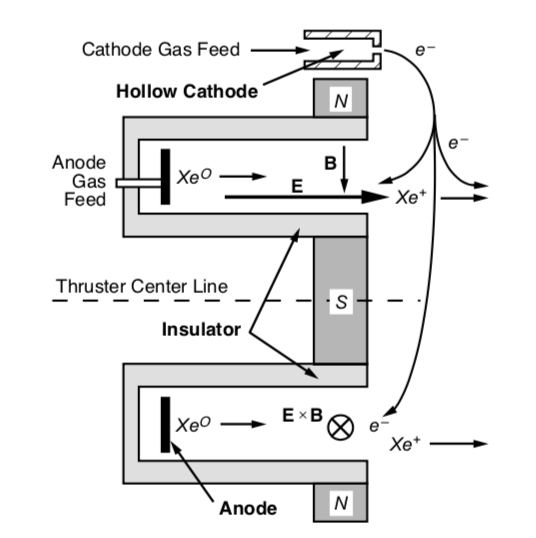
\includegraphics[width= 0.5\textwidth]{hall_thruster}
\caption{\label{fig:hall_thruster} Schematic cross section of a typical Hall thruster \cite{goebel}}
\end{figure}

Gas is fed into the discharge channel through the anode and dispersed into the channel. Electrons attempting to reach the anode encounter a transverse radial magnetic field, which reduces their mobility in the axial direction and inhibits their flow to the anode. The electrons tend to spiral around the thruster axis in the $E \times B$ direction and represent the Hall current after which the device is named. Ions generated by these electrons are accelerated by the electric field from the anode to the cathode-potential plasma produced at the front of the thruster. Some fraction of the electrons emitted from the hollow cathode also leave the thruster with the ion beam to neutralize the exiting charge. The shape and material of the discharge region channel and the details of the magnetic field determine the performance of the thruster.

\subsection{Building a Hall Thruster}

Hall thrusters are the dominant electric propulsion technology in use today. Fabrication of an industrial grade Hall thruster begins with a finite element analysis of the magnetic field required to meet the thrust specifications, and can be carried out using the Finite Element Method Magnetics software found online \cite{femm}. This gives the dimensions of the thruster that needs to be built. A thermal analysis is then conducted to ensure that the materials used can withstand the high voltages and propellant pressure involved.\\

The best materials to build the channel and cathode are ones that work best in the presence of plasma. Boron nitride and alumina are ideal for this, and can be procured in the United Kingdom from Good Fellow Ceramics or Precision Ceramics. The anode requires a refractory metal like tungsten or molybdenum, and require custom suppliers for fabrication. The 3D files and the material specifications can then be sent to the suppliers mentioned above, who can professionally machine all the parts required.\\

\begin{figure}[h!]
\centering
\includegraphics[width= 0.7\textwidth]{hall_industrial}
\caption{\label{fig:hall_industrial} Schematic of an industrial grade Hall thruster}
\end{figure}

A makeshift thruster can be built in a well equipped laboratory using the following methods:

\begin{itemize}
\item The anode can be fabricated using CNC machined aluminium.
\item The cathode can be built from 0.5mm thick thoriated tungsten wire which would generate electrons when a current is passed through it. This cathode could also be used to neutralize the plume.
\item The channel can be constructed from a 3D printed RTV silicone template which could be used to mould 50\% Plaster of Paris (POP).
\item For the propellant, krypton could be used as a viable alternative to xenon since it is 10 times cheaper and delivers the requisite ionization. The propellant can be sourced from BOC gases in the UK, and the amount of propellant needed (about 250g) can be worked out from the mass flow rate. A pressure regulator (down to 1 bar) with a quarter inch swagelok connector would be required to ensure proper flow of the propellant into the channel.
\end{itemize}


However, since fabrication of an industrial grade thruster is far beyond the scope and timeline of this project, a combination of ion thruster design form factor and electro-hydrodynamics has been used to build the thruster for this project \cite{prototype}.


%\pagebreak
\subsection{Corona Discharge}

Corona discharge refers to the phenomenon when the electric field near a conductor is strong enough to ionize the dielectric surrounding it but not strong enough to cause an electrical breakdown or arcing between conductors or other components. This phenomenon is unwanted and dangerous in high-voltage systems; however, a controlled corona discharge may be used to ionize a fluid and induce motion by directly converting the electrical energy into kinetic energy.\\

The potential at which corona originates is called the corona threshold voltage or corona inception voltage. Above this voltage, there is a limited region within which current increases linearly with voltage. This is known as the Ohm’s law regime. Beyond this region, current increases more rapidly and ultimately leads to arcing at the breakdown potential.\\

\begin{figure}[h!]
\centering
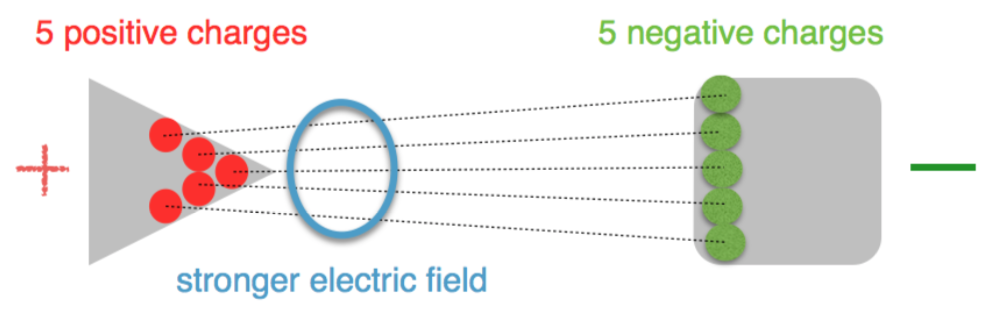
\includegraphics[width= 0.75\textwidth]{corona_1}
\caption{\label{fig:corona_1} Illustrating the difference in the electric field around sharp points. \cite{workshop}}
\end{figure}

The electric field intensity is higher around the surface of a charged conductor with higher curvature or lower radii of curvature. If Q is the total charge stored in a conductor and r is its radius of curvature, the electric field intensity E is inversely proportional to the radius according to:

\begin{equation}
E = \frac{Q}{4 \pi \epsilon_0 r}
\end{equation}


where $\epsilon_0$ is the permittivity of free space (and air, since the relative permittivity of air is 1.0006) and is equal to $8.852 \times 10^{-12}$ F/m.\\

As the electric field intensity increases, it affects electrons in the atomic orbitals and may cause atoms to release electrons. The maximum electric field that a dielectric material can withstand without conduction is called the dielectric strength of that material, and is often expressed in V/mm. When the electric field increases beyond this maximum point, the material becomes conducting due to the avalanche effect. In this case, electrons collide with the atomic or molecular structure, releasing more electrons which in turn lead to further breakdown of the material.\\

Breakdown is usually accompanied by large currents. The dielectric strength of air at normal temperature and pressure is \textbf{3 kV/mm}. At this point, air ionizes rapidly and arcing occurs. This is what happens during a lightning strike. However, corona discharge occurs below the breakdown potential, which is why there is no significant damage to the material.\\


An electron that is excited by an electric field E will ionize an atom or molecule of a gas if it has enough energy. This energy threshold is called the ionizing potential of the particular gas, and is expressed in eV. However, if the electron does not have enough energy, it will impart a certain amount of kinetic energy to the particle it collides with. The kinetic energy gained by the atom is released as photons which have a specific energy and wavelength. This results in the glow associated with corona discharges.\\

When corona discharge is induced across two similar electrodes, it is called a bipolar corona. If one of the electrodes has a lower radius of curvature compared to the other, a uni-polar corona is formed since the corona discharge would be almost completely concentrated around the electrode with higher curvature. This electrode is called the active electrode. If the active electrode is made positive with respect to the passive electrode, a positive corona discharge occurs. If the active electrode is made the cathode, a negative corona is generated.\\

Corona can be generated by a high AC or DC voltage. If an AC voltage is used, it can be sinusoidal or pulsed. Tesla coils generate strong corona discharge effects and operate at high frequencies of about 300 kHz. Corona has been found to be \textbf{more intense at higher frequencies}. Pulsed power is especially preferred for industrial applications. In the case of pulsed power discharges, the \textbf{duty cycle} of the waveform can be modified to alter the \textbf{power consumption} or the \textbf{rate of ionization}. The DC offset can also be altered to vary the effects.



\subsection{Ionocraft: Electrohydrodynamic Ion-Propelled Aircraft}
\label{ehd_ionocraft}

Electrohydrodynamics (EHD), also known as electro-fluid-dynamics or electrokinetics, is the study of the dynamics of electrically charged fluids. It involves analyzing the motions of ionized particles or molecules and their interactions with electric fields and the surrounding fluid.\\

A popular application of EHD is the lifter shown in Figure \ref{fig:lifter}. It has no moving parts. Instead, the surrounding fluid is ionized and accelerated by a high potential gradient to generate an ionic wind. An ionic wind results from the net momentum gain in a mostly neutral fluid through momentum-transfer collisions with ions in an electric field.\\

\begin{figure}[h!]
\centering
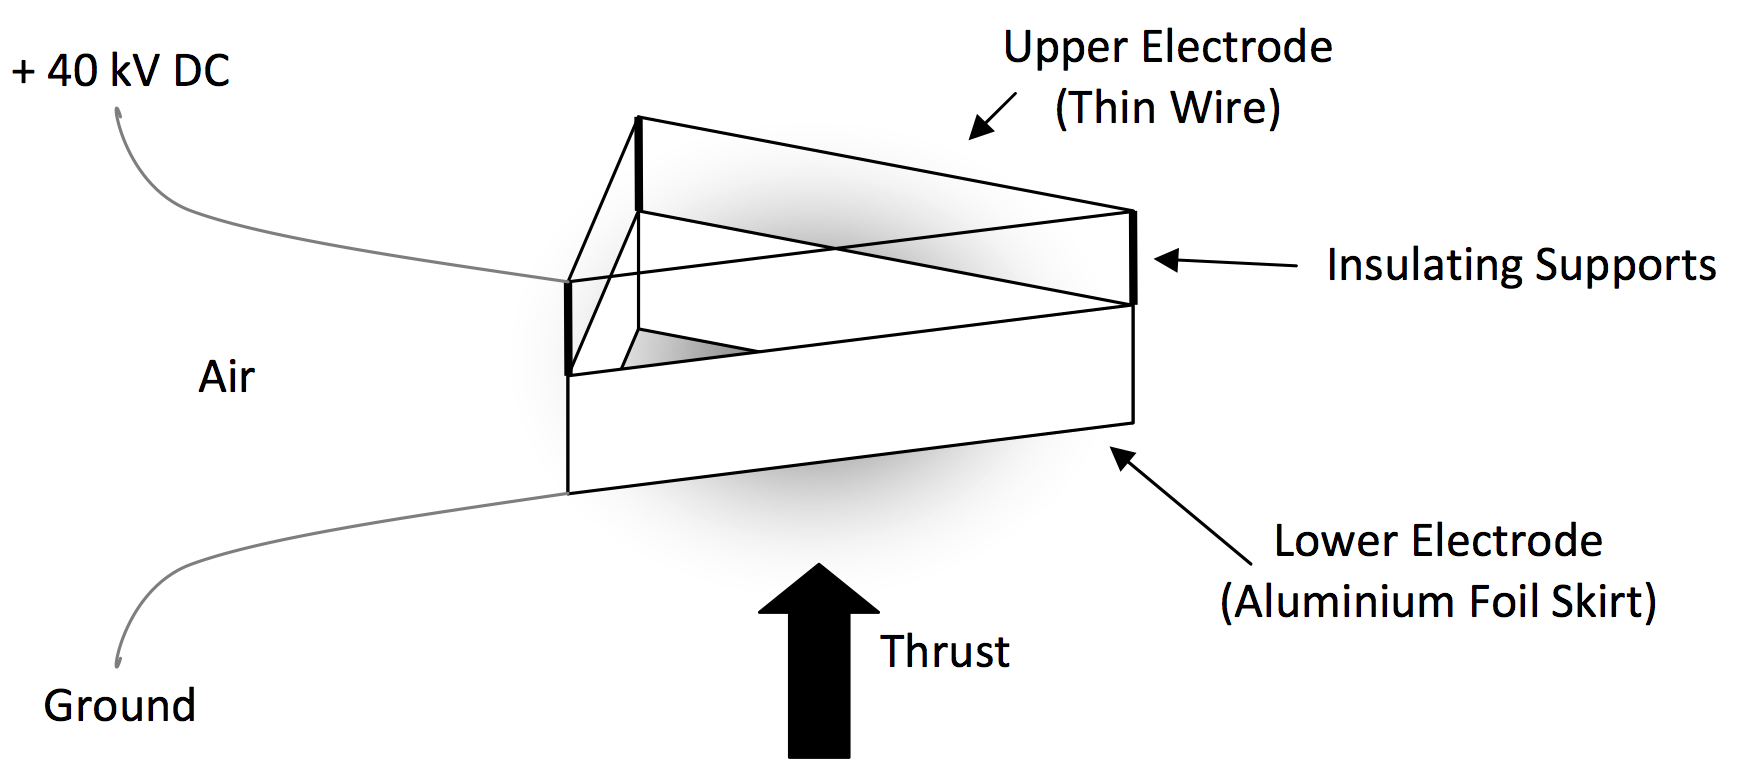
\includegraphics[width= 0.9\textwidth]{lifter}
\caption{\label{fig:lifter} Schematic of a basic ionocraft \cite{ehdperform}}
\end{figure}

When a voltage in excess of the corona inception voltage (Vo) is applied across two electrodes with different radii of curvature, a non-uniform electric field with the largest magnitude in the vicinity of the smaller emitter electrode ignites a corona discharge that emits an ion stream. The ions are then transported across the interelectrode gap at an average drift velocity $v_D = \mu E$, where $\mu$ is the ion mobility and E is the electric field magnitude. The ions are collected at the collector electrode and do not contribute to thrust, but the neutral air molecules that gained energy in the collisions along the way escape the system with net momentum along the direction from the emitter towards the collector. This produces thrust in the opposite (i.e upward) direction.\\

\begin{figure}[h!]
\centering
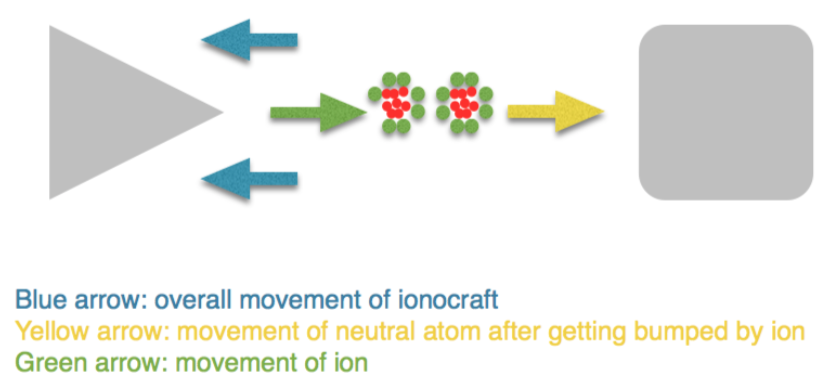
\includegraphics[width= 0.7\textwidth]{corona_3}
\caption{\label{fig:corona_2} Illustrating the direction of thrust due to corona discharge. \cite{workshop}}
\end{figure}

Single stage thrusters (shown in Figure \ref{fig:lifter}) refer to an arrangement of using one emitter electrode, an air gap and a collector electrode with a larger radius of curvature than the emitter. Double stage thrusters add a collinear intermediate electrode. For single stage thrusters, increasing the gap length requires a higher voltage for thrust onset, generates less thrust per input voltage, generates more thrust per input current and most importantly generates more thrust per input power. Double stage thrusters have been shown to be more effective than their single stage counterparts at producing current, leading to a smaller total voltage necessary for producing equal thrust. However, losses involving ion collection at the intermediate electrode lead to reduced thrust-per-power compared to a single stage thruster of equal length.\\

\begin{figure}[h!]
\centering
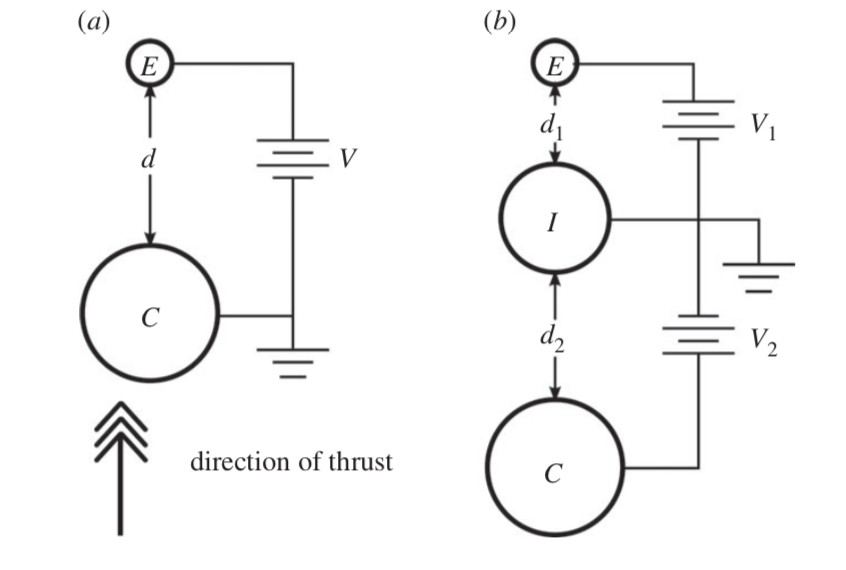
\includegraphics[width= 0.6\textwidth]{ss_ds}
\caption{\label{fig:ss_ds} Equivalent circuits for single and double stage ionocrafts. \cite{ehdperform}}
\end{figure}

Although scientists have been experimenting with this kind of propulsion since the 1960s, it hasn't been applied to large scale aircraft yet due to power concerns. However, in 2013, scientists at the Massachusetts Institute of Technology (MIT) built a working prototype that delivered a thrust of 110 Newtons per kilowatt - far higher than the 2 Newtons per kilowatt generated by a jet engine \cite{mit}. Since the craft is silent, has zero emissions, and has no infrared signature, there are a number of potential military and security applications. Unlike the traditional ion thruster, the ionocraft needs air molecules for propulsion which makes it useful only within an atmosphere \cite{verge}. This atmosphere need not be that of Earth, and the ionocraft can be used for exploration of other planets where an all-electric propulsion without moving parts may be beneficial.


\subsection{Thrust to Power Ratio of a Single Stage Ionocraft}
\label{tp_ratio}

An expression for thrust in terms of current throughput can be calculated using the following assumptions:

\begin{enumerate}
\item The electrode length is long compared to the gap length d and electrode radii.
\item Space charge effects are low at corona ignition and hence neglected. However it will become more pronounced as current and charge density increase.
\end{enumerate}

Defining current density using the ion drift velocity and a characteristic area A perpendicular to x, the total current is:

\begin{equation}
I = \int j \cdot dA = \int \rho \mu E \cdot dA = \rho \mu EA
\end{equation}

where $\rho$ is the charge density. The thrust is then equal to the Coulomb force on the volume of ions occupying the gap at any instant in time:

\begin{equation}
F = \int \rho E dV = \int_0^d \rho E \cdot A dx = \frac{Id}{\mu}
\end{equation}

The voltage-current relationships for corona discharges are as follows \cite{ehdperform}:

\begin{equation}
I = CV(V-V_0)
\end{equation}

where $V_0$ is the corona inception voltage and $C \propto \frac{\mu}{d^2}$.\\

Therefore the thrust can be expressed as a function of voltage:

\begin{equation}
F_{SS} = \frac{C'V(V-V_0)}{d}
\end{equation}

where C' is an empirical value dependent on geometry.\\

The input power is simply the product of the current and voltage output of the power supply. Therefore the thrust to power ratio is:

\begin{equation}
\frac{F}{P_{SS}} = \frac{Id}{\mu IV} = \frac{d}{\mu V}
\end{equation}
\\

While this equation implies that efficiency improves with the electrode gap d, the electric field needs to be strong enough to cause corona discharge and yet low enough to avoid breakdown. There would be no lift if these conditions are not met. The equations above also demonstrate how thrust and efficiency can be varied for a given gap d. For example, a higher voltage would lead to higher thrust but low efficiency and vice versa.\\




\pagebreak
\section{Design and Construction}

The following flow chart presents an overview of the main parts of the prototype:

\begin{figure}[h!]
\centering
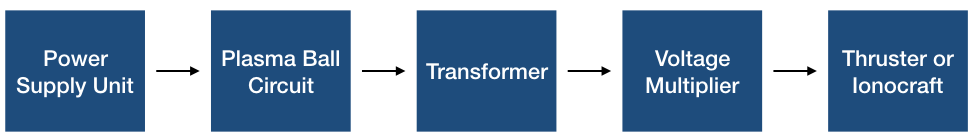
\includegraphics[width= \textwidth]{flow}
\caption{\label{fig:flow} Overview of the prototype's main stages}
\end{figure}

\subsection{The Power Supply}

The main constraint imposed on this project is that the bench power supply unit (PSU) provided by the Imperial College electrical engineering undergraduate laboratory needs to be used instead of a high voltage direct current (HVDC) power supply in order to meet the safety standards of the project. Any voltage boost provided must be carried out within an enclosed box placed on the apparatus for safety. Therefore, a means of stepping up the input voltage to the order of a few kilovolts (while adhering to the given constraints) is required before any measurable thrust can be observed.\\

Any power supply used for this project needs to meet a few key criteria:

\begin{enumerate}
\item It needs to provide a stable high voltage DC output that can be continuously varied as required for testing.
\item The output current needs to be limited so that the equipment isn't damaged in case of an accidental short circuit.
\item The output voltage and current should be easily measurable to a reasonable degree of precision.
\item It must be built within the limited budget requirements of the project.
\item It should be safe for people and equipment operating in the surrounding area. 
\item It should be easy to use and maintain.\\
\end{enumerate}


Most available AC to DC converters and switch mode power supplies are easy to make, but usually operate below 200V DC. Building an HVDC supply involves a number of challenges, including procuring components rated at the required voltages and currents, ensuring proper insulation, and isolation of stages. Many commercial suppliers manufacture HVDC supplies, but they usually cost a few thousand dollars. Common household appliances like Cathode Ray Tube (CRT) televisions, computer monitors, microwave ovens, automobile ignition systems can be fashioned into usable HVDC supplies, but have their limitations.\\

Some of the options explored for this project were \cite{panicker}:

\begin{enumerate}
\item \textbf{Van de Graaff generator}: An electrostatic generator that builds a static charge on a sphere from a rolling belt made of a non-conducting material such as rubber or nylon. They are capable of generating voltages up to 20 MV using very low currents ($\mu A$ or lower). However, the output voltage drops as the current is drained, so it is not a viable DC source.
\item \textbf{Tesla Coil}: Tesla coils generate high AC voltages at hundreds of kilohertz. The primary and secondary LC circuits can be tuned by varying the turns ratio, and at the right frequency, a standing wave is amplified to a large voltage at the secondary. However, it is difficult to control the output voltage and rectify it to a steady DC level.
\item \textbf{Fly Back Transformers (FBT)}: The transformer could be used to step up the commonly available mains voltage (240 V at 50 Hz) before rectification with diodes. FBTs are used to accelerate the electron beam in  cathode ray tubes found inside old televisions and computer monitors, and usually operate from a few kHz to the lower MHz at around 30 kV. However the circuit inside is not isolated or insulated enough to meet the saferty standards of the project.
\item \textbf{Microwave Oven Power Supply}: These are usually capable of producing 2 to 3 kV at 1 to 4 kW and are used to power the magnetron that produces the microwaves to heat food. Therefore multiple stages would need to be cascaded in order to meet the requirements of this project, which would be dangerous since the insulation may not be able to withstand voltages higher than the device's rating. Unlike FBTs, this supply is not current limited by saturation of the core which makes it dangerous in case of a short circuit in the secondary coil.
\item \textbf{Ignition Transformer}: Fuel oil ignition transformers are used in fuel oil burning heaters to ignite fuel with an arc, and are usually rated at 10 kV, 20 mA. Although this is current limited by the core, the secondary windings can burn in case of a short circuit in the secondary coil. Automobile ignition transformers can produce 30 kV AC but require a complex circuit to produce a variable output. Therefore although they are cheap, they are not a good choice for an HVDC supply.
\item \textbf{Neon Transformer}: These are used to produce luminescence in luminescent tubes and commercial displays by exciting low pressure inert gases with a high voltage. Since the AC mains voltage is connected to the AC generator via an isolation transformer (1:1 turns ratio), the high voltage side is isolated from the line. The output is then connected to a bridge rectifier and filtered with a capacitor. Therefore this is a viable option for the project. However, the device could not be procured in time for the project. 
\end{enumerate}

Since all of the above options had some drawback or the other, the final design choice was to use the bench power supply unit, the circuit from a Plasma Ball and a voltage multiplier in order to achieve the required output voltage.

\pagebreak
\subsection{The Plasma Ball Circuit}

\begin{figure}[h!]
\centering

\includegraphics[width= 0.9\textwidth]{plasmaball}
\caption{\label{fig:plasmaball} Overview of the plasma ball circuit}
\end{figure}

The circuit from a Global Gizmos plasma ball \cite{plasmaball} has been used to provide the first voltage boost. The DC output from the bench PSU was soldered to the input on the ball's printed circuit board (PCB). An oscillator on the PCB generates a square wave to switch a Darlington pair, which converts the PSU's DC input into a square wave for the transformer. The Darlington's current amplification and higher collector voltage provide an increased power input to the transformer. Remember the transformer needs a varying input to successfully step up the voltage.\\

When the base voltage of the Darlington goes high, the collector voltage drops. This causes the magnetic field inside the transformer to collapse. The coils in the transformer react according to Lenz's law to maintain the input voltage at the transformer (i.e the collector voltage of the Darlington), which in turn provides a surge in the transformer's output voltage due to the turns ratio. When the base goes low, the collector voltage rises again, and the transformer output gradually reduces. This output is then fed to a Cockroft Walton voltage multiplier for a further boost.

\begin{figure}[h!]
\centering
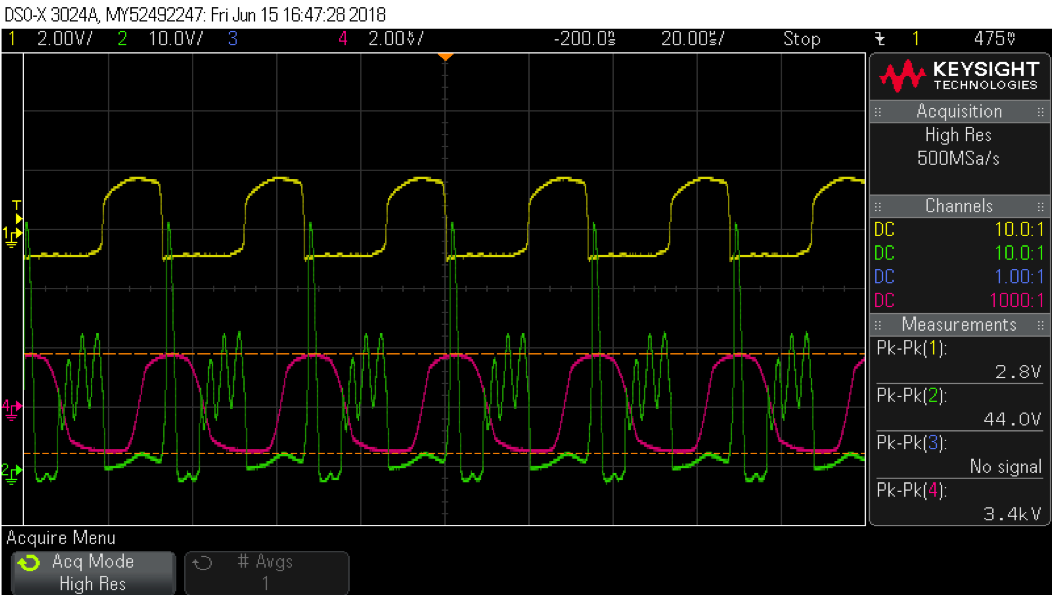
\includegraphics[width = 0.8\textwidth]{thruster_sc_1}
\caption{\label{fig:transformer_out} Scope reading showing the driver voltage, collector voltage, and transformer output.}
\end{figure}

\pagebreak
\subsection{The Cockcroft-Walton Voltage Multiplier}

The Cockroft Walton circuit is a ladder network of capacitors and diodes that generates a high voltage DC signal from a low voltage AC input. It is lighter and cheaper than a transformer since it does not need a heavy core or extensive insulation and uses relatively low cost components. The output can be tapped from any stage like a multi-tapped transformer.\\

\begin{figure}[h!]
\centering

\includegraphics[width= 0.6\textwidth]{cockroft}
\caption{\label{fig:cockroft} A 2 stage Cockroft Walton voltage multiplier circuit}
\end{figure}

Figure \ref{fig:cockroft} shows a 2 stage multiplier. Assume all capacitors are uncharged initially, and that the alternating input voltage $V_i$ has a peak value of $V_p$. When the input reached $-V_p$, current flows through diode $D_1$ to charge capacitor $C_1$ to a voltage of $V_p$. When $V_i$ becomes $+V_p$, it adds to $C_1$'s voltage to give $2V_p$ on the right hand plate. $D_1$ is now reverse biased, so current flows from $C_1$ through $D_2$ to charge $C_2$ to 2$V_p$.\\

The next time $V_i$ changes polarity, current flows from $C_2$ through $D_3$ to charge $C_3$ to 2$V_p$. Similarly the next polarity change causes current from $C_3$ to flow through $D_4$ to charge $C_4$ to 2$V_p$. In this way, current flows through the ladder with each change in polarity until the entire network is charged. All capacitors have a voltage of $2V_p$, except for $C_1$, which has a voltage of $V_p$. The trick used here is that although the capacitors are charged in parallel, they are connected to the load in series. Therefore the total voltage across $C_2$ and $C_4$ is $V_o = 4V_p$.\\

The ladder can be extended to any number of stages. The number of stages is the number of capacitors in series between the output and ground. This gives the output voltage:

\begin{equation}
V_o=2NV_p=NV_{pp}
\end{equation}

where $V_{pp}$ is the peak to peak input voltage.\\

As the number of stages increases, the voltage output of the later stages "sags" due the impedance of the lower stage capacitors. When supplying an output current, the voltage ripple increases with the number of stages. Therefore, the Cockroft Walton multiplier is generally used when a low output current is required. if required, these effects can be reduced by increasing the capacitance of the lower stages, increasing the input power frequency, and using an AC power source with a square or triangular waveform.\\

The \textbf{5 stage} multiplier used in this project was constructed using 1 nanofarad 15 kilovolt ceramic disc capacitors and 15 kilovolt 550 milliamp standard recovery microwave oven diodes in order to withstand the large voltages and power dissipation involved, providing a stable maximum output voltage of \textbf{20 kV}. In order to be practical for an ion propulsion engine, the multiplier needs to be light. This can be accomplished by driving it from a high frequency source such as an inverter or a high voltage transformer, which significantly reduces the physical size and weight of the circuit.



\subsection{The Thruster}

The thruster consists of 2 components: an anode and a cathode. The exact dimensions of its various parts are shown in the figure below. Note that this is neither a Hall thruster nor an ion thruster, but an application of EHD propulsion using the same form factor as an ion thruster.\\

\begin{figure}[h!]
\centering
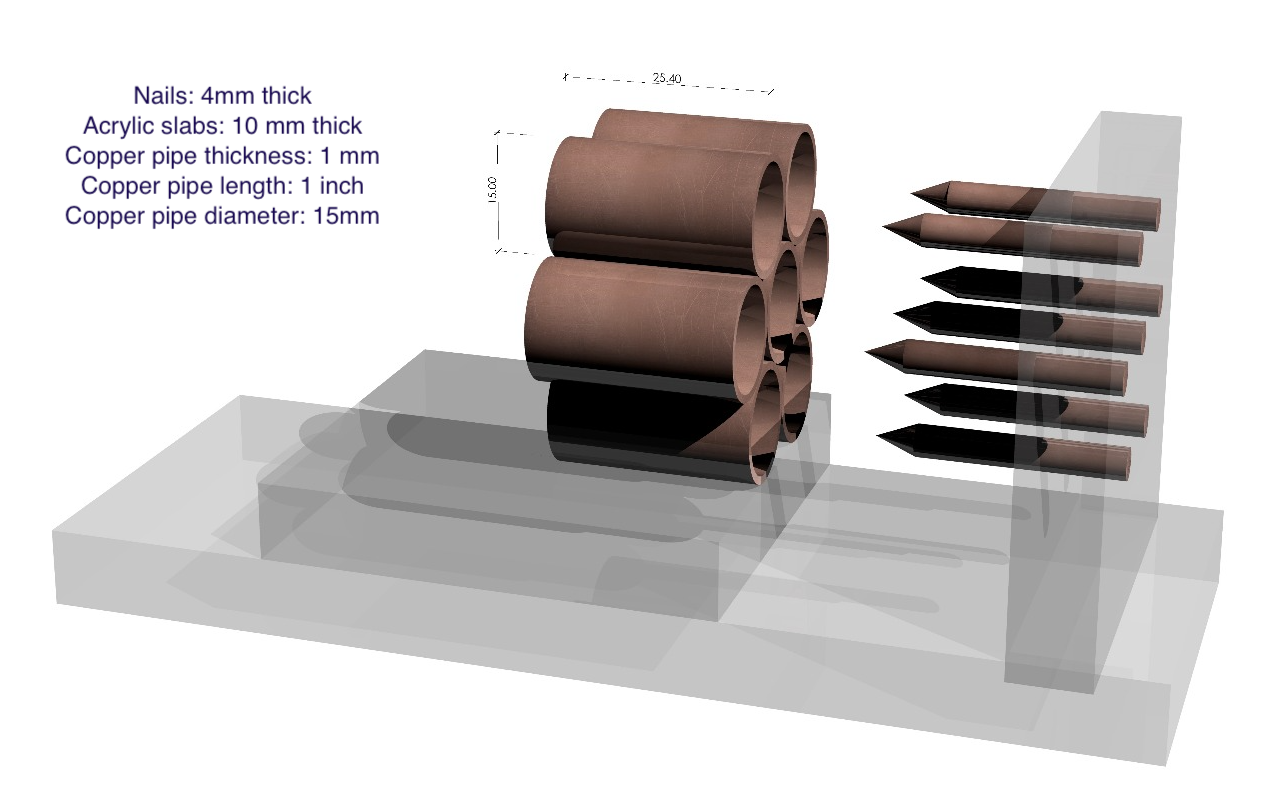
\includegraphics[width = 0.8\textwidth]{thruster_schematic}
\caption{\label{fig:thruster_schematic} A 3D rendering of the thruster's design.}
\end{figure}

The cathode consists of 7 copper pipes arranged in a beehive pattern. A pipe cutter was used to obtain 6 one inch long sections. A generous amount of flux paste was applied between the pipes to fuse them together and form an electrical connection. They were then held in the beehive formation by an aluminium ring and further secured by nichrome wire. These were chosen since their soldering temperature is much higher than that of copper.\\

\begin{figure}[h!]
\centering
\begin{subfigure}{0.32\textwidth}
\centering
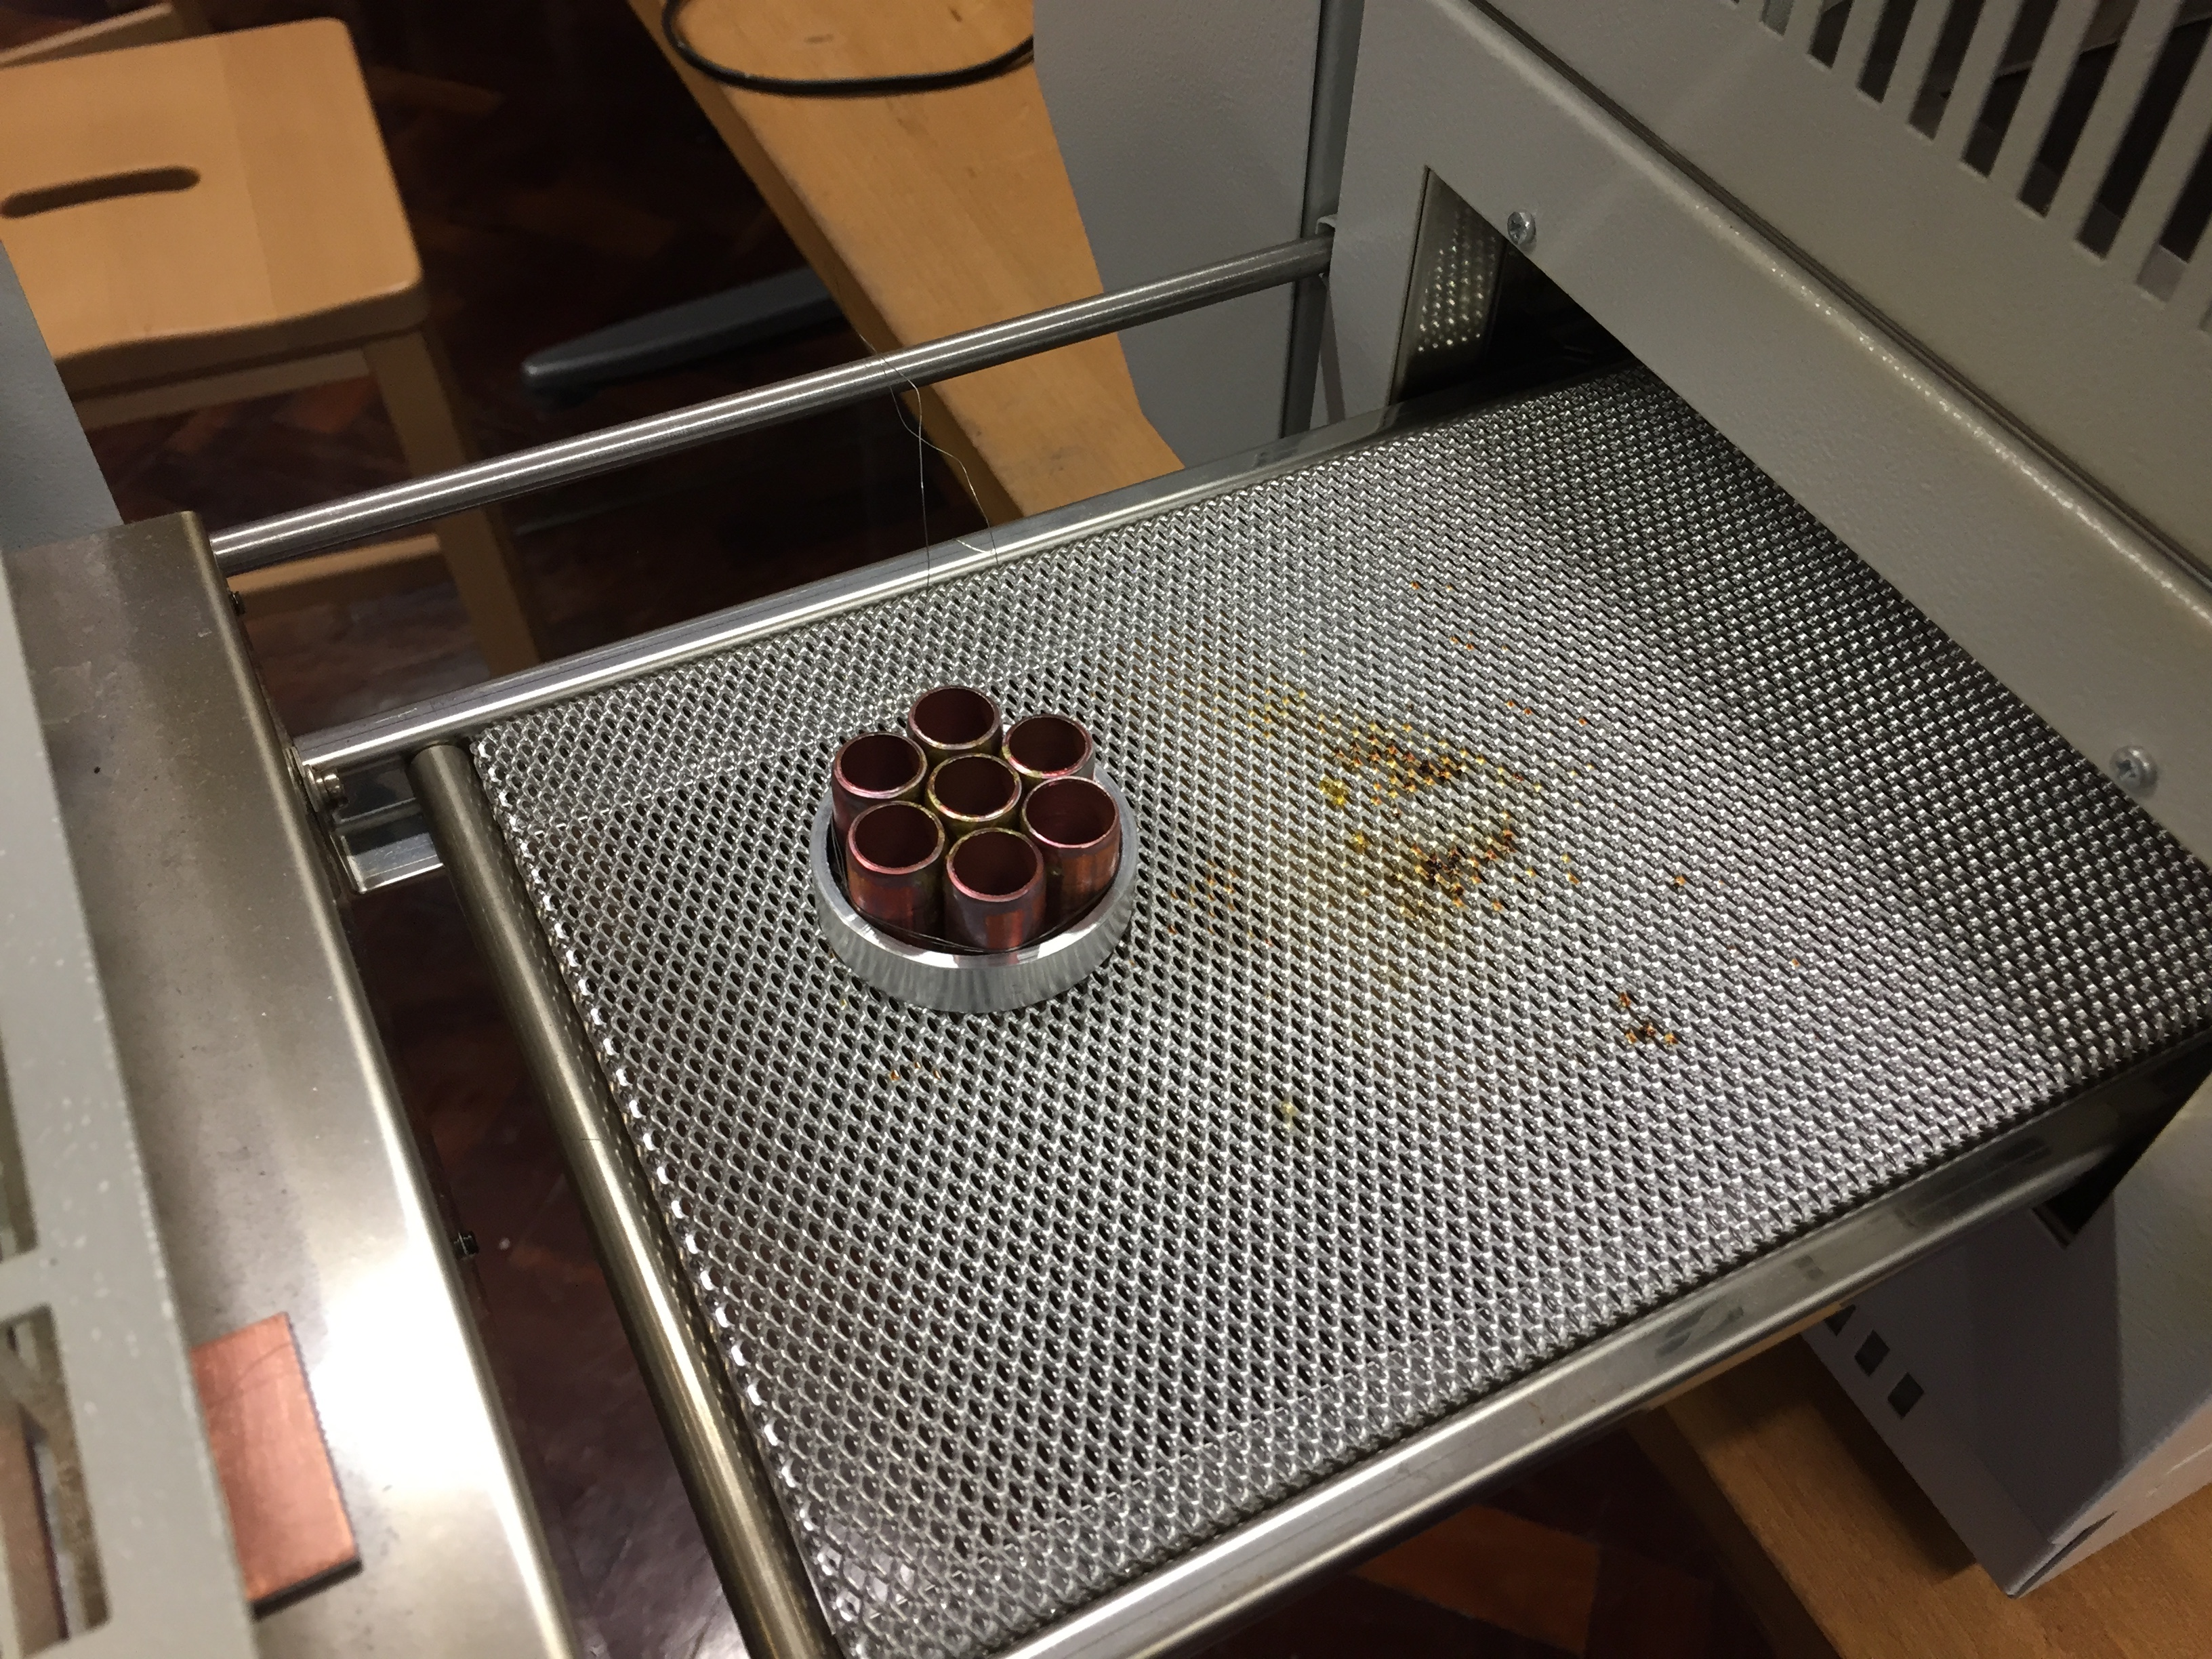
\includegraphics[width = \textwidth]{thruster_1}
\caption{}
\label{fig:thruster_1}
\end{subfigure}
\begin{subfigure}{0.32\textwidth}
\centering

\includegraphics[width = \textwidth]{thruster_2}
\caption{}
\label{fig:thruster_2}
\end{subfigure}
\begin{subfigure}{0.3\textwidth}
\centering
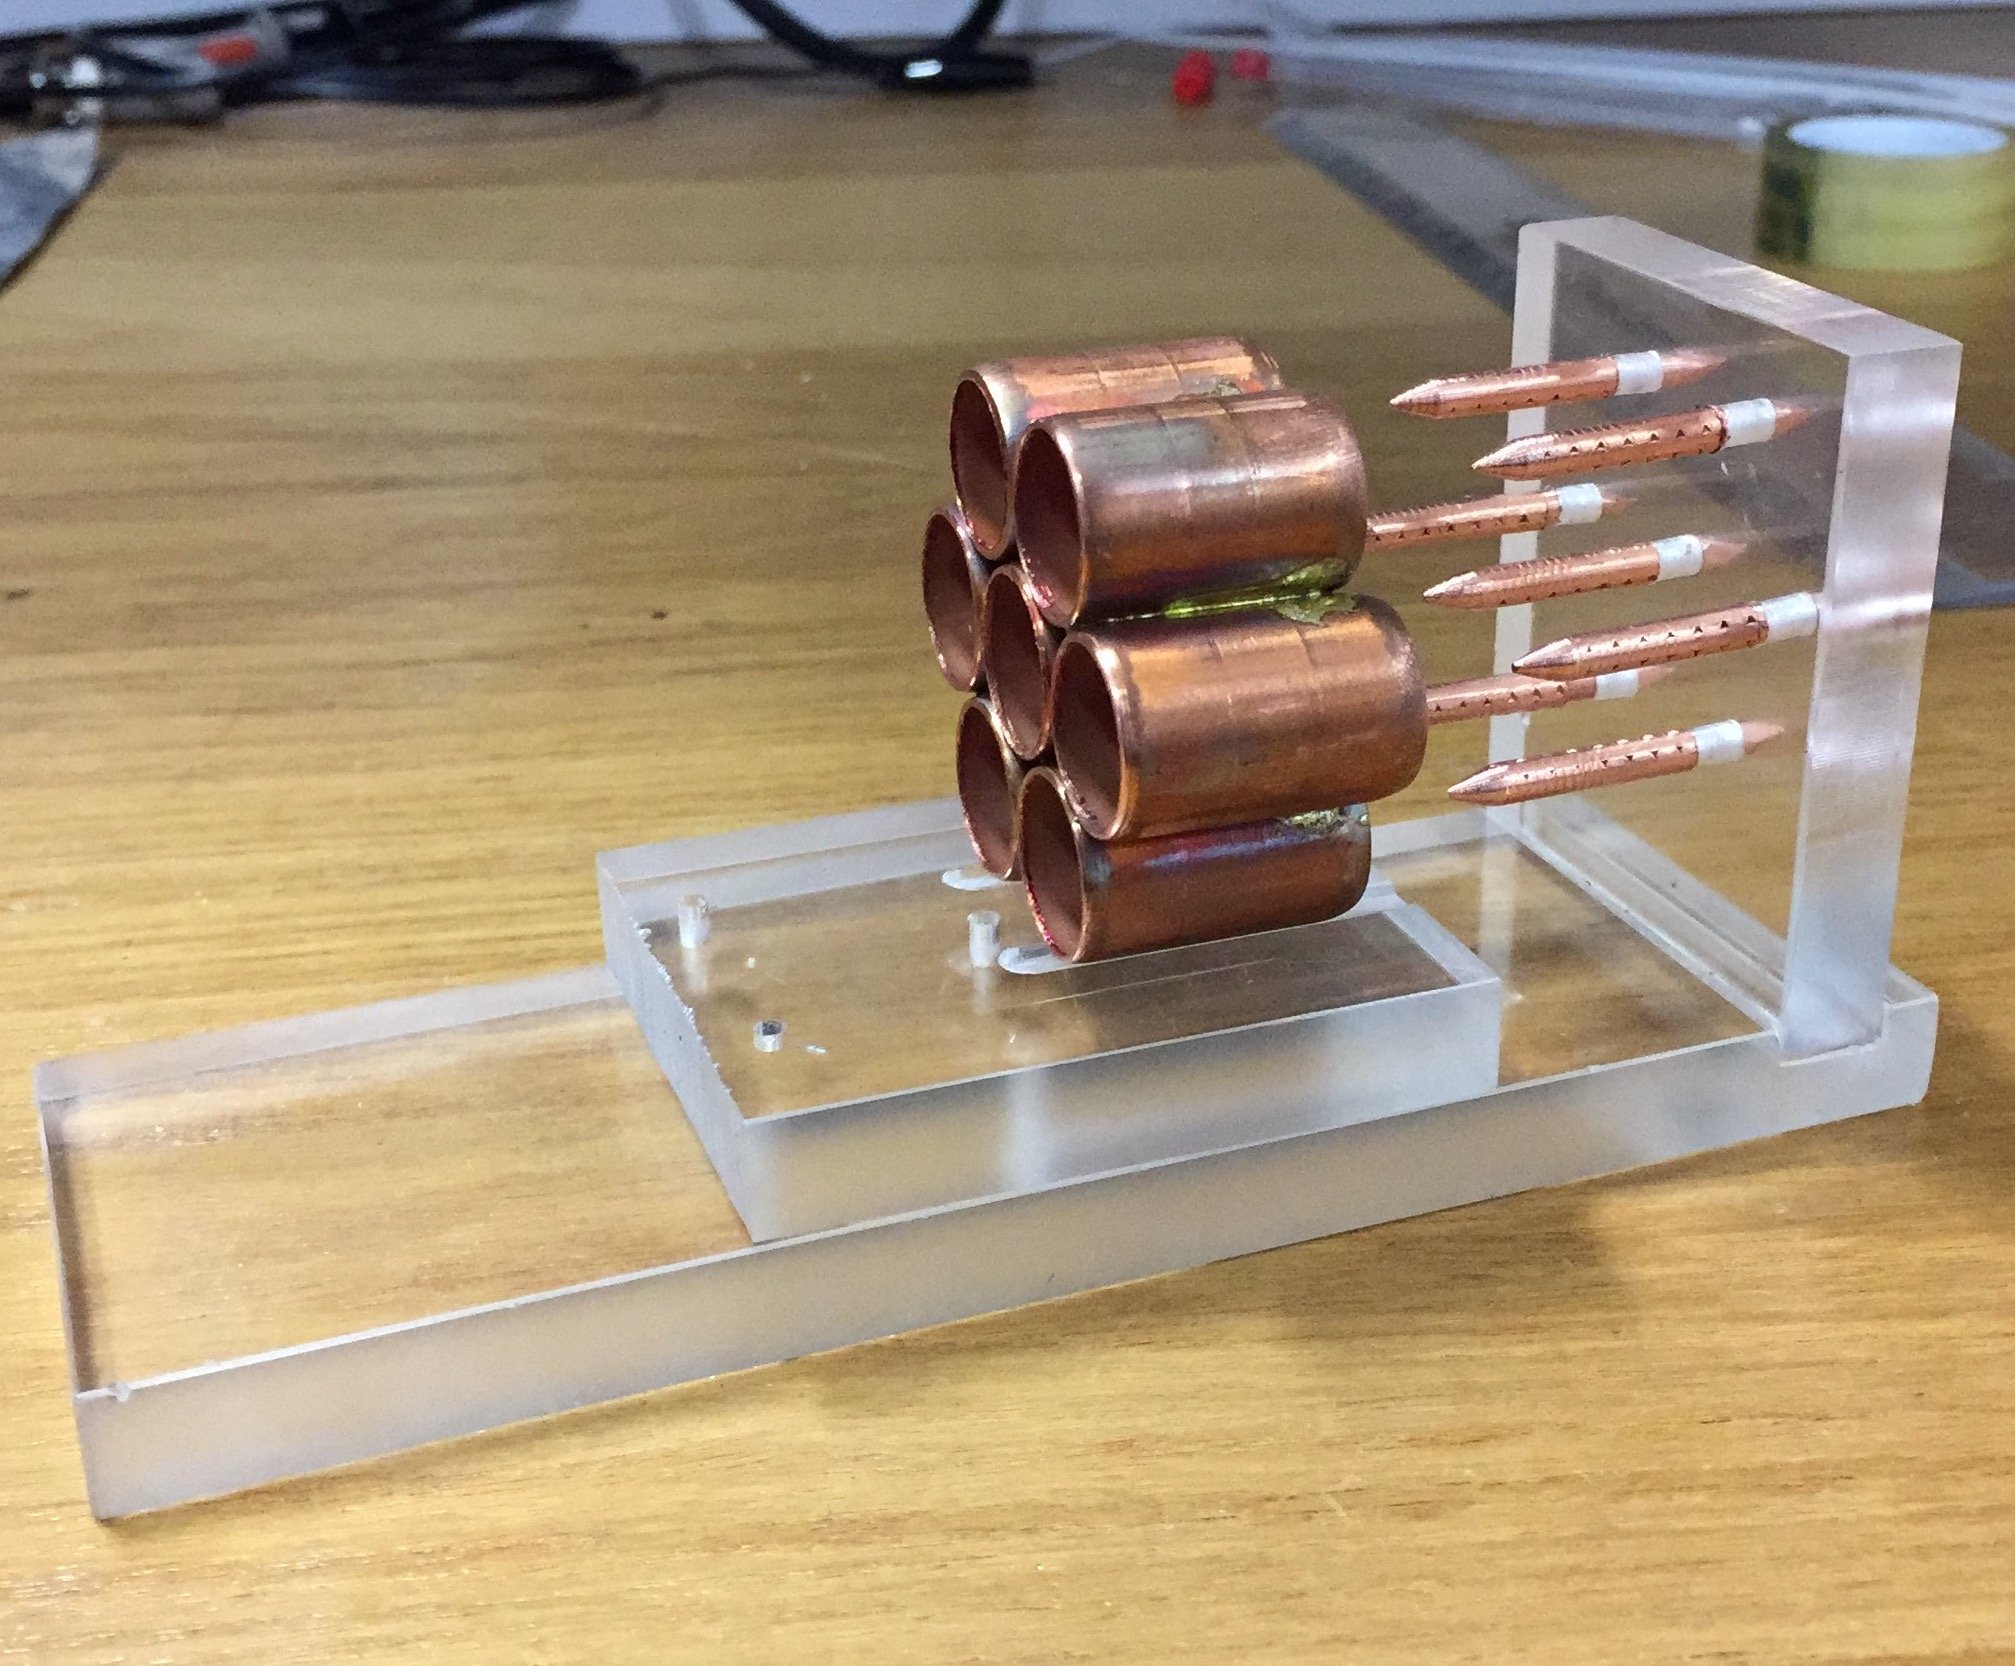
\includegraphics[width = \textwidth]{thruster_3}
\caption{}
\label{fig:thruster_3}
\end{subfigure}
\caption{\label{fig:thruster_construct} Building the thruster}
\end{figure}

The traditional way to fuse the pipes is to use a blowtorch. However, since the mechanical workshop was out of propane, a reflow soldering machine used to heat surface mounted printed circuit boards (PCBs) was used instead. After preheating the oven to 260 degrees Celsius,  the secured pipes were placed inside for 4 minutes, after which another 10 minutes were allowed to cool them. The solder melted completely, forming an excellent electrical connection between the pipes as well as a strong physical bond. This structure is placed on a small acrylic slab taped onto the larger base slab. The use of tape allows the distance between the cathode and the anode to be varied as required.\\

The anode consists of an acrylic slab with 7 copper nails  drilled through it. Each nail is arranged to be in line with the centre of its corresponding copper tube in the cathode, and the back of the nails are soldered to a single wire to form a continuous electrical connection. However, the nails proved to be too thick for effective corona discharge, so they have been used as mounts for 35 SWG wires with their insulation removed at one end. This bunch of wires is then connected at the other end to the output of the voltage multiplier through a high voltage cable.

\subsection{The Ionocraft}

The design used is the same as that shown in Section \ref{ehd_ionocraft}, which consists of 3 main parts.\\

\begin{figure}[h!]
\centering
\begin{subfigure}{0.32\textwidth}
\centering
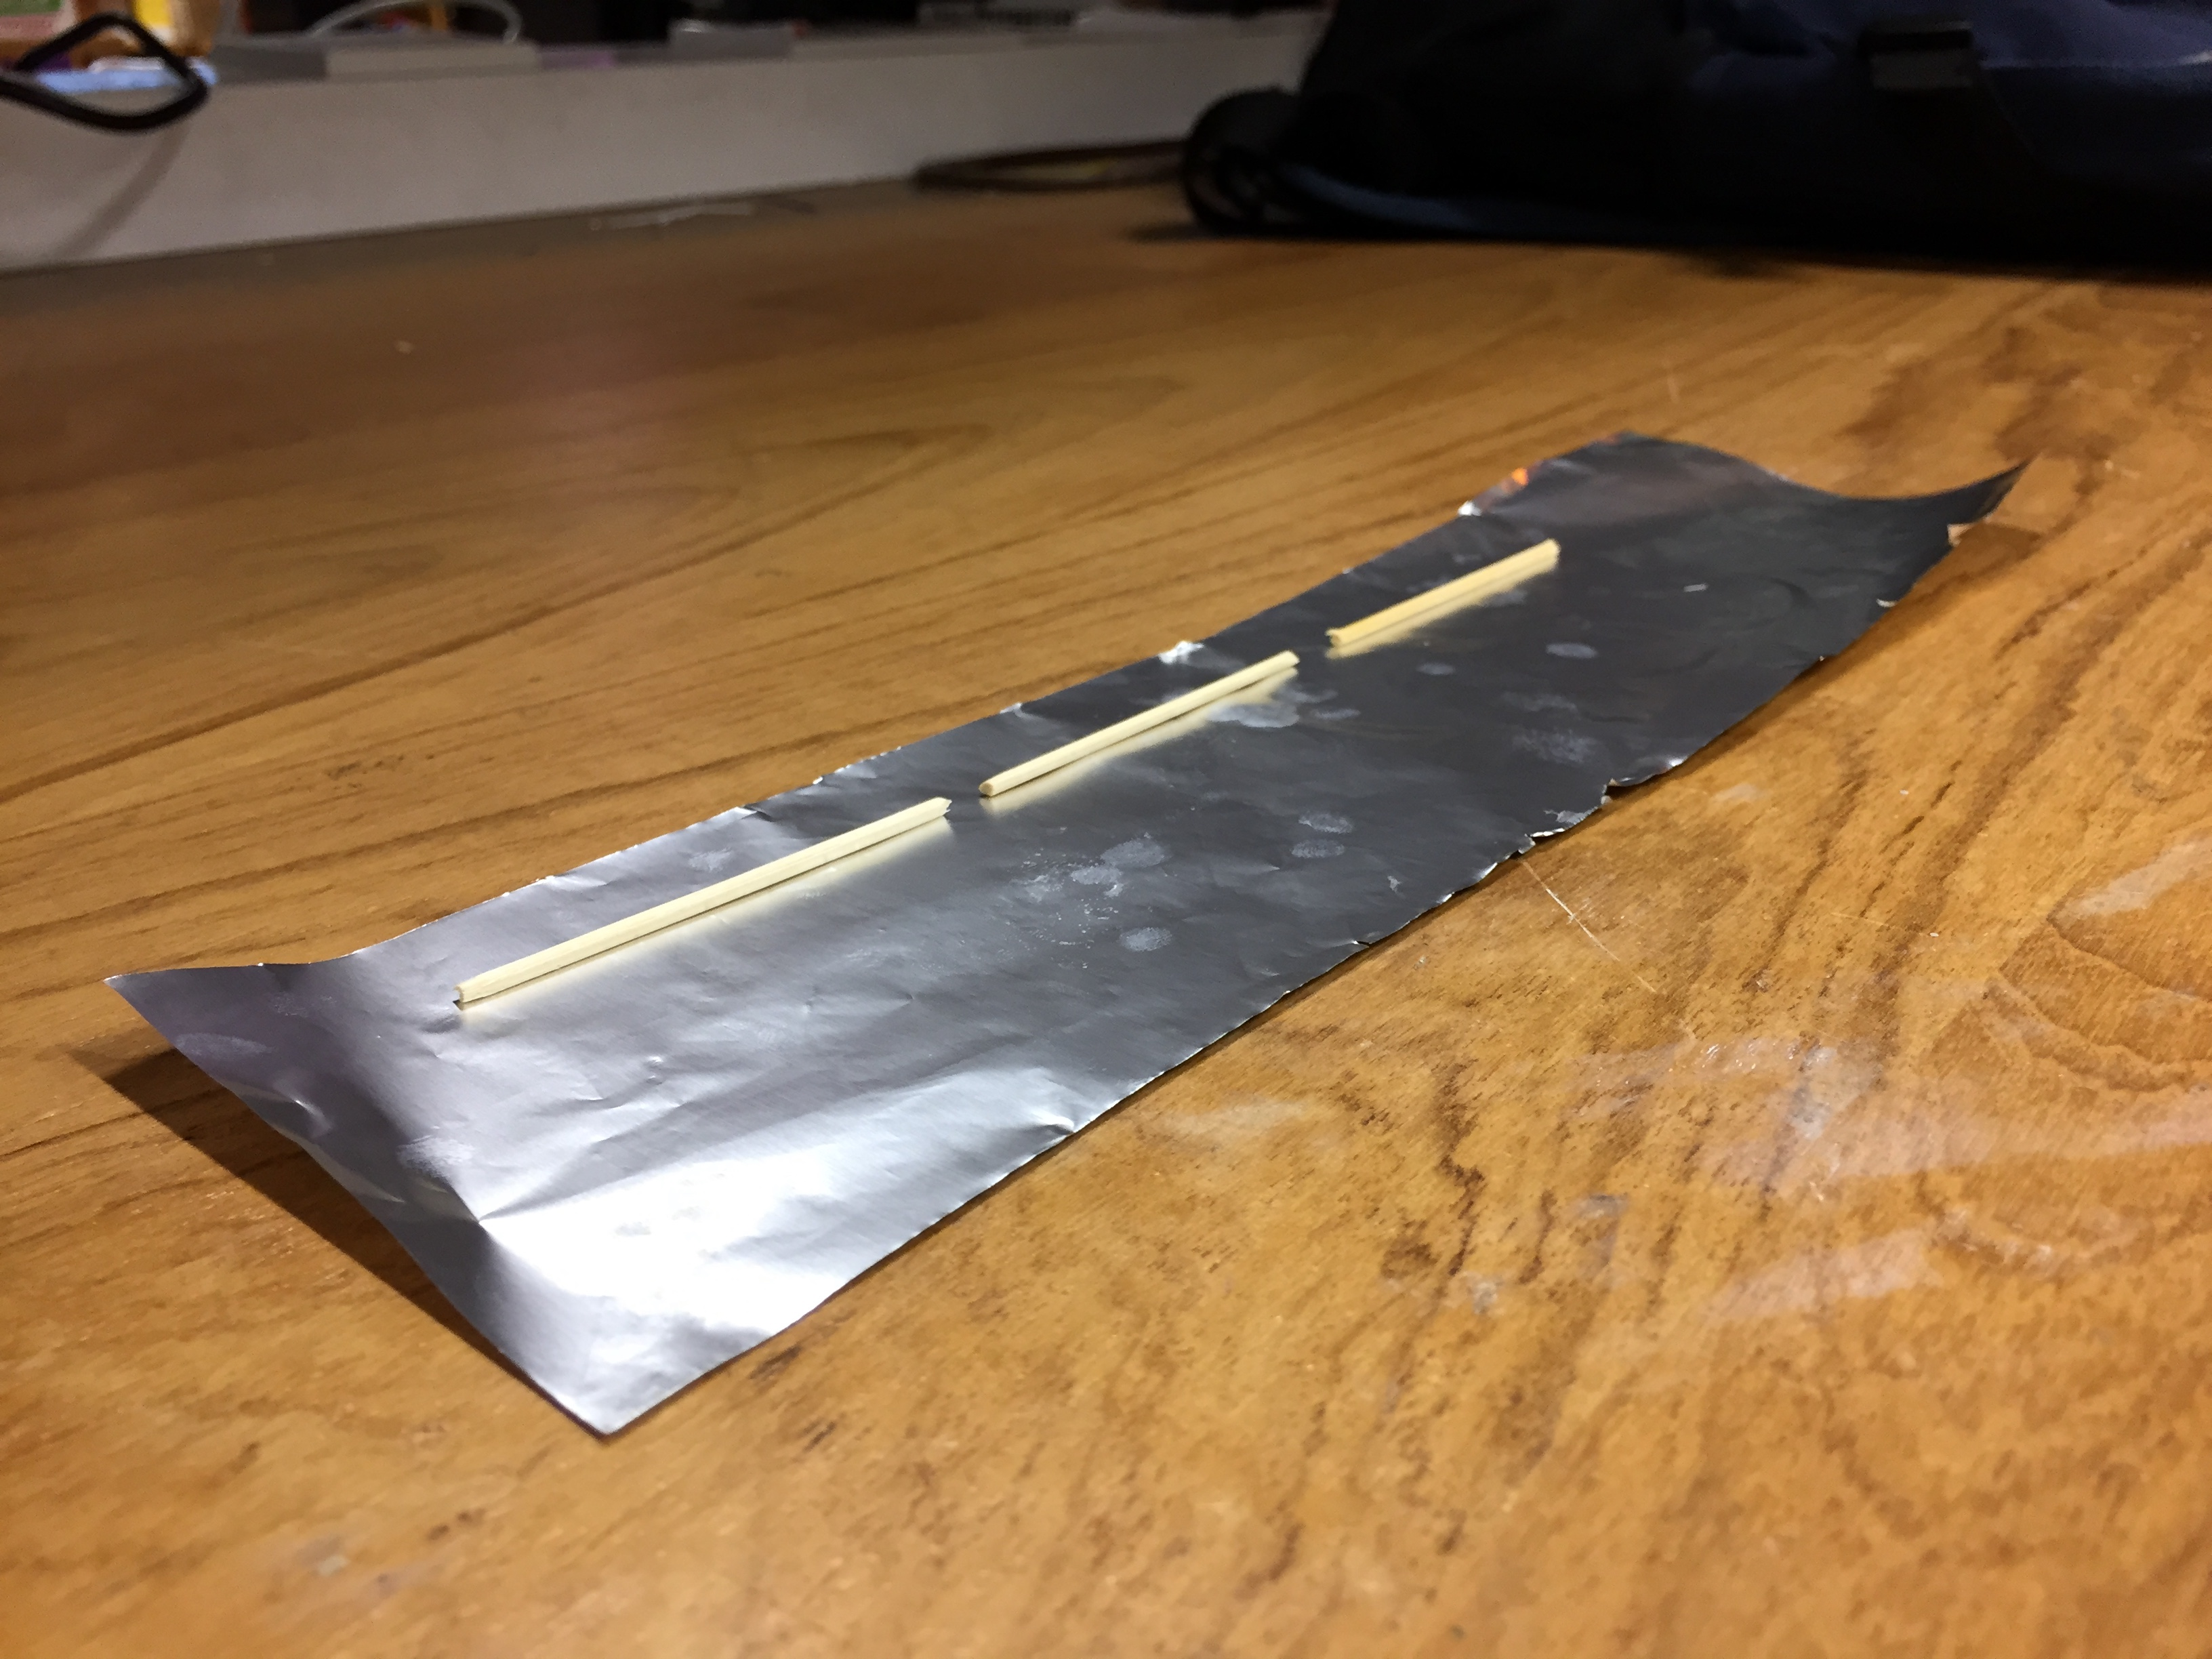
\includegraphics[width = \textwidth]{craft_1}
\caption{}
\label{fig:craft_1}
\end{subfigure}
\begin{subfigure}{0.32\textwidth}
\centering
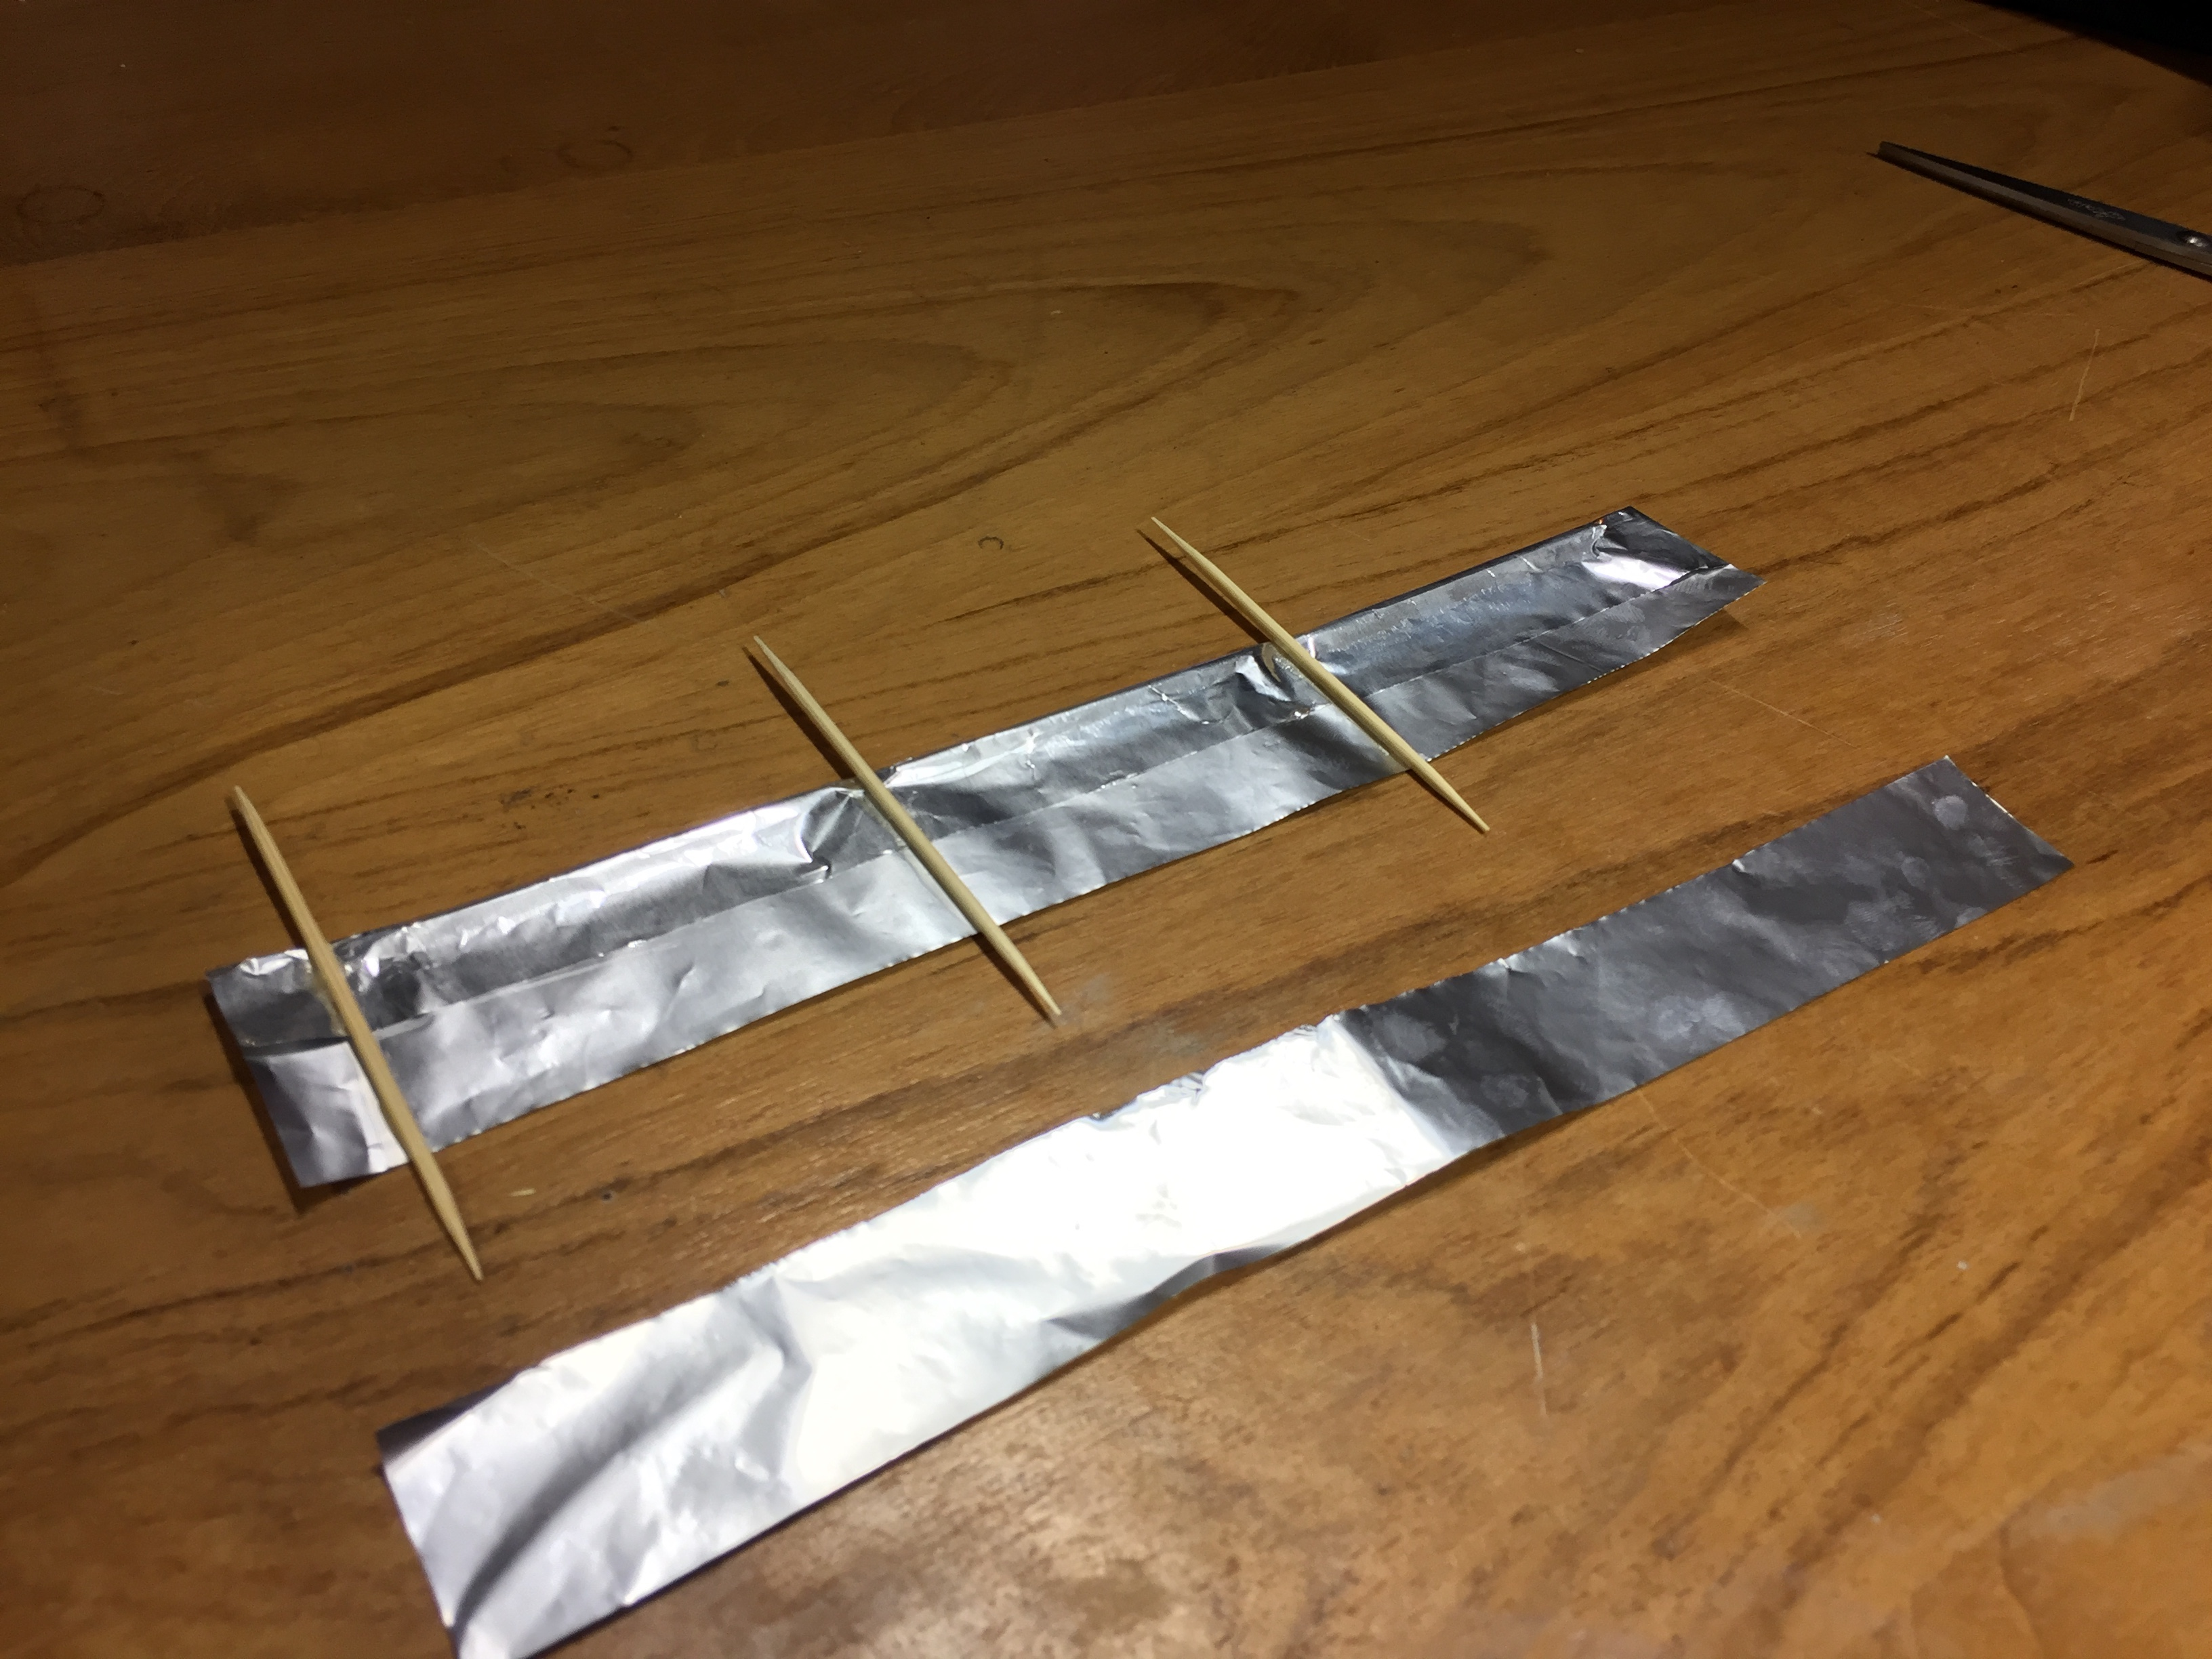
\includegraphics[width = \textwidth]{craft_2}
\caption{}
\label{fig:craft_2}
\end{subfigure}
\begin{subfigure}{0.32\textwidth}
\centering
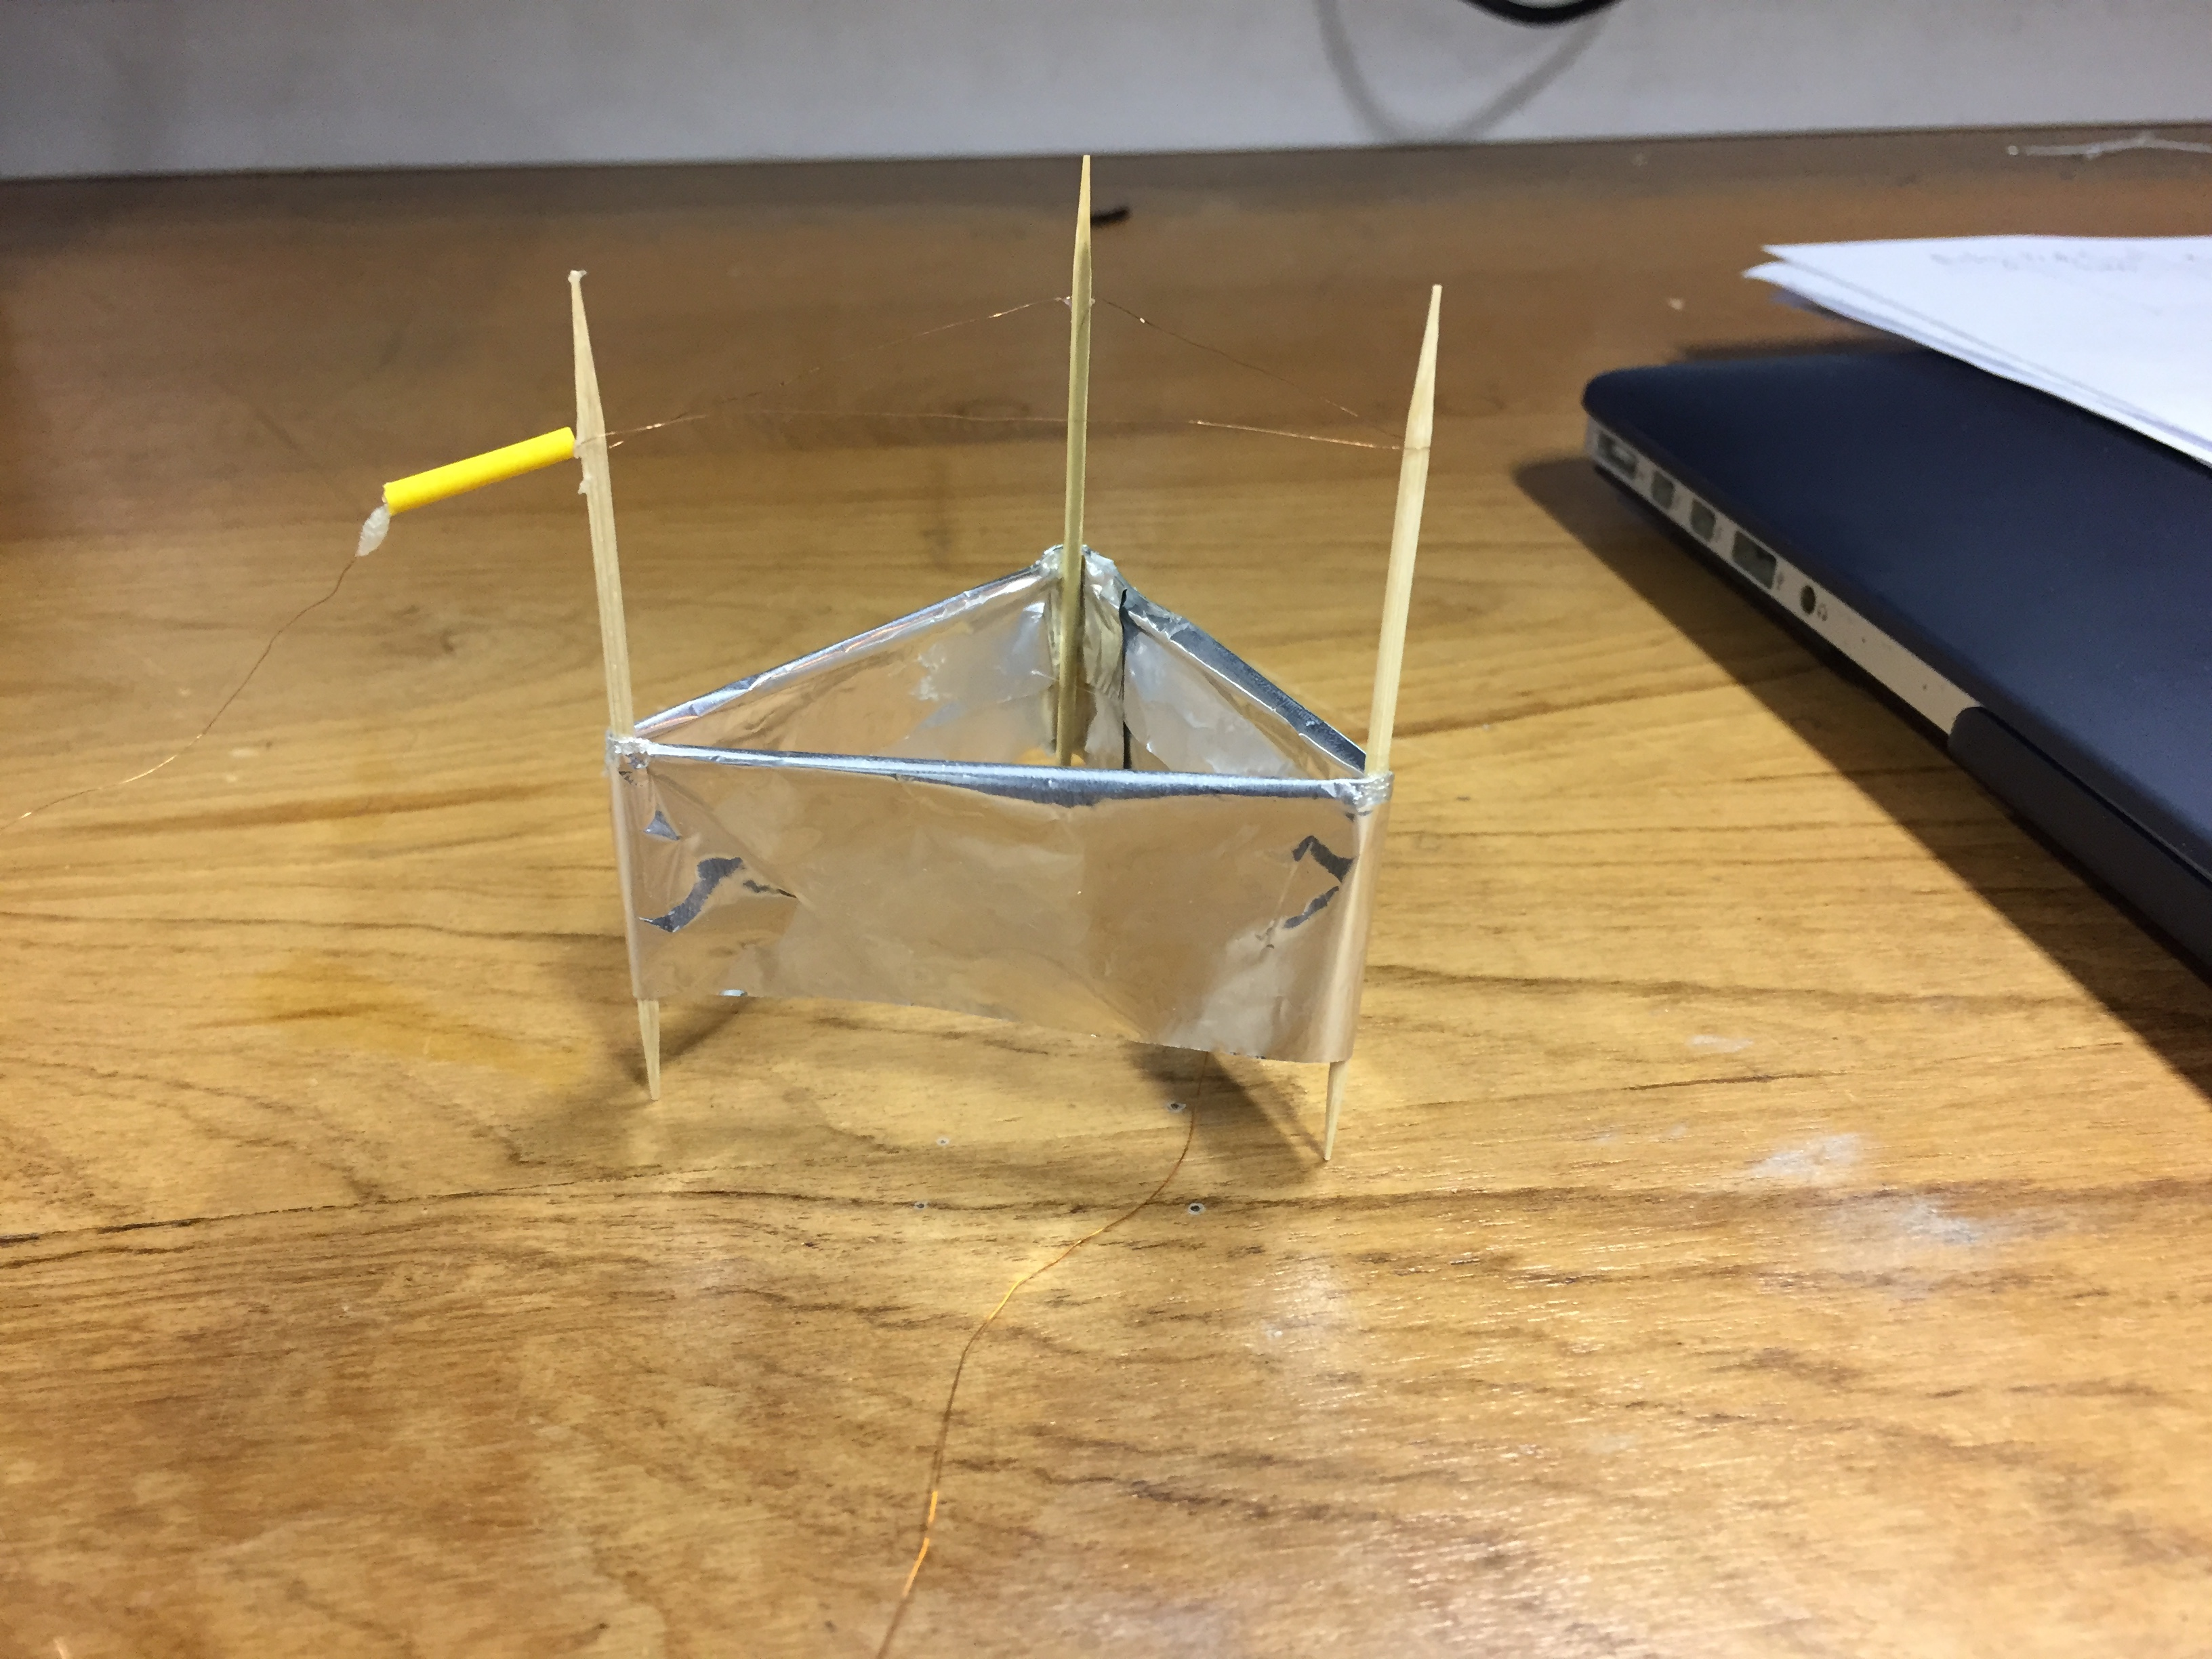
\includegraphics[width = \textwidth]{craft_3}
\caption{}
\label{fig:craft_3}
\end{subfigure}
\caption{\label{fig:craft_construct} Building the ionocraft}
\end{figure}

The first is the 42 SWG (0.1 mm thick) wire tied around 3 vertical cocktail sticks. This wire is connected to the high voltage supply (voltage multiplier output or directly to the HVDC supply). The wire is the sharp body from which ions are released via corona discharge, and thus needs to be bare (without insulation) and as thin as possible.\\

Removing the insulation throughout the length of such a thin wire was too cumbersome, so the required length was pulled from the intertwined copper wires in the sheathing of a coaxial cable. 30 gauge wire was experimented with as well, but it proved to be too heavy and did not release enough ions to generate lift. The wire must be moved up or down along the vertical supports in order to find the perfect trade off between spreading of dissipated ions (if it is too far away from the receiving electrode) and arcing (if it is too close to the receiving electrode).\\

The second component of the craft is its skeleton. This includes the vertical cocktail sticks (each measuring 8 cm in length) mentioned earlier as well as 3 more horizontal sticks that provides the necessary curvature to the aluminium foil that forms the receiving electrode. A variety of options including straws and plastic ink refills were experimented with to form a supporting structure, but the cocktail sticks provided the best combination of low weight and rigidity. The sharp ends of the horizontal sticks were clipped to avoid tearing the foil.\\

The third part of the craft is the receiving electrode, for which a long strip of Sainsbury's Basics kitchen foil has been used. The aluminium skirt was 8 cm by 2 cm, and held one centimeter above the ground. One end of a thin wire was stripped of its insulation and then taped to the foil opposite to the joint connected to the positive high voltage supply. The other end of this wire was connected to ground. While the craft will operate even if the polarities are reversed, keeping the high voltage electrode away from the surface simply reduces the risk of a short circuit.\\

Before the craft can operate as intended, a few adjustments need to be made to prevent arcing and maximize thrust. The overhead wire must be as straight as possible and follow the triangular aluminium skirt below. Any sharp metal points in the circuit are sources of ions, so all the soldered connections need to be smoothened out. The short length of bare wire connecting the craft to the high voltage supply was covered with insulation, and the soldered joint was covered in glue. The 3 corners of the craft had sharp points where the aluminium folded, so they were covered in glue to prevent conduction. Care had to be taken not to add too much weight so as to hinder lift off.


\subsection{Safety Precautions}

Since the project uses lethal levels of current (i.e greater than 0.1 amperes), a few important precautions were taken:

\begin{enumerate}
\item The workspace was a large, low traffic, cordoned off area in order to minimize possible accidents.
\item The apparatus was only operated in the vicinity of a trained technician.
\item The apparatus was only be operated within its nominal range, was always safely discharged before approaching it, and was left unplugged if there was no operator near its power cord.
\item The apparatus was always covered entirely by a large plastic storage box during any experiments in order to protect users against any possible sparks.
\item A flat head metal pin was hammered into one end of a large wooden stick and then soldered to an earth connection. This stick served as a means of discharging high voltage points from a distance.
\item The various stages of the voltage multiplier were discharged after every test in case any of the soldered connections had become loose during testing.
\item A current limiting power supply was used in order to prevent any dangerous current surges. The current level was always monitored while conducting experiments. 
\item The oscilloscope was always kept on to monitor the driver, collector and transformer output voltage in order to notice any changes due to the transistor overheating.
\item A high voltage probe was always connected to the voltage multiplier output to ensure the thruster or the ionocraft was completely discharged before touching it.
\end{enumerate}
 

\pagebreak
\section{Testing}

In order to vary the input frequency and duty cycle, we disconnect the oscillator from the plasma ball circuit and feed the Darlington with a function generator. An RS Pro weighing scale with a resolution of 1mg has been used to measure thrust output, and the readings have been scaled to millinewtons. Note that the thrust follows the current trend almost exactly in all the following tests, which is exactly as we would expect from the derivation in Section \ref{tp_ratio}.

\subsection{The Thruster}

\subsubsection{Varying Input Power}

\begin{figure}[h!]
\centering
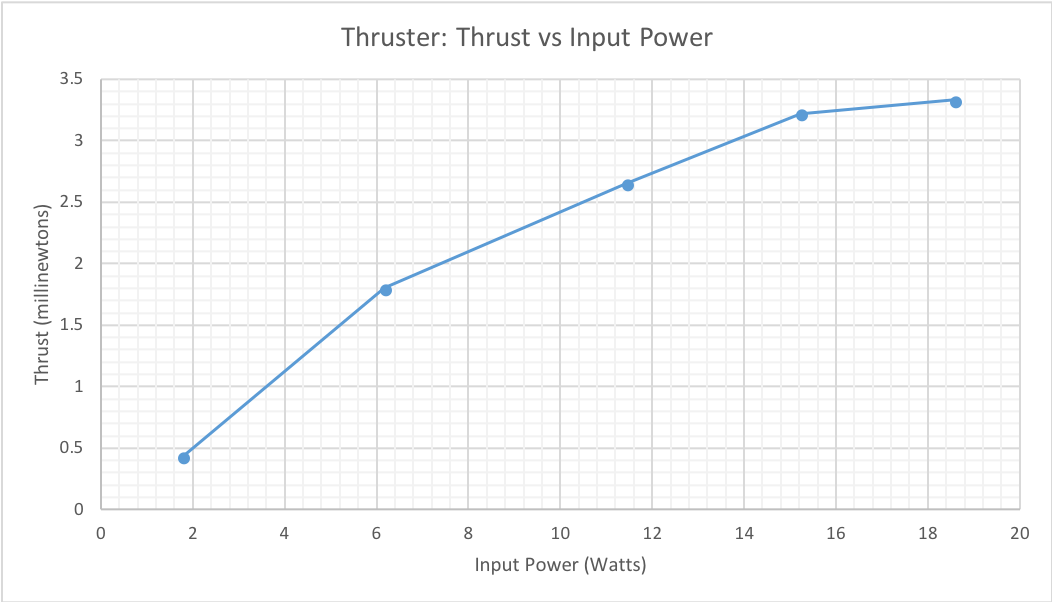
\includegraphics[width = 0.8\textwidth]{thruster_g1}
\caption{\label{fig:thruster_g1} Relationship between thrust and input power for the stationary thruster}
\end{figure}

\begin{figure}[h!]
\centering
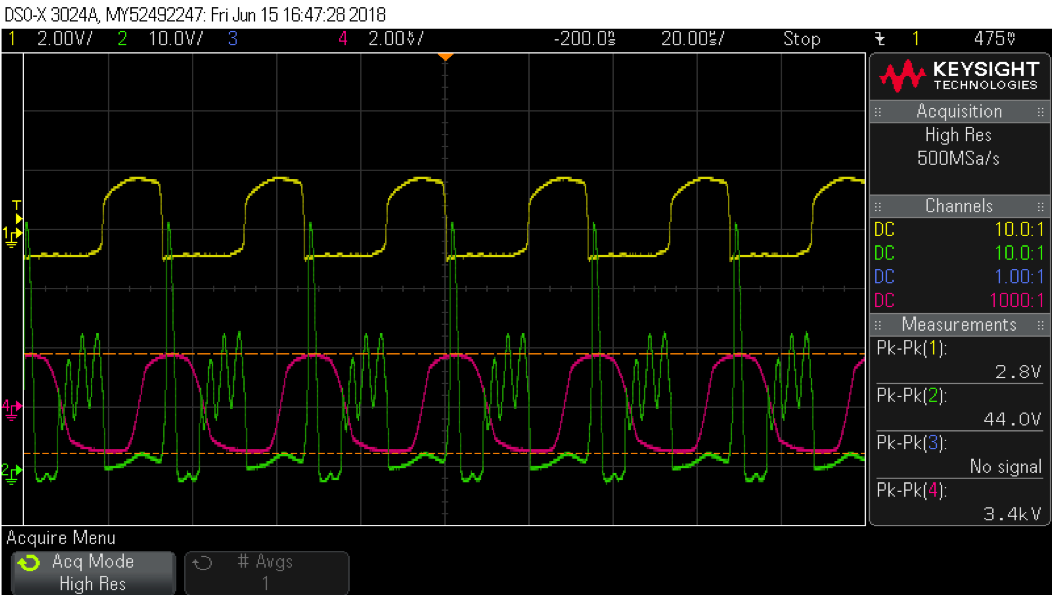
\includegraphics[width = 0.8\textwidth]{thruster_sc_1}
\caption{\label{fig:thruster_sc_1} Scope reading showing the driver voltage, collector voltage, and transformer output for the thruster}
\end{figure}


\pagebreak
\subsubsection{Varying Input Duty Cycle}

\begin{figure}[h!]
\centering
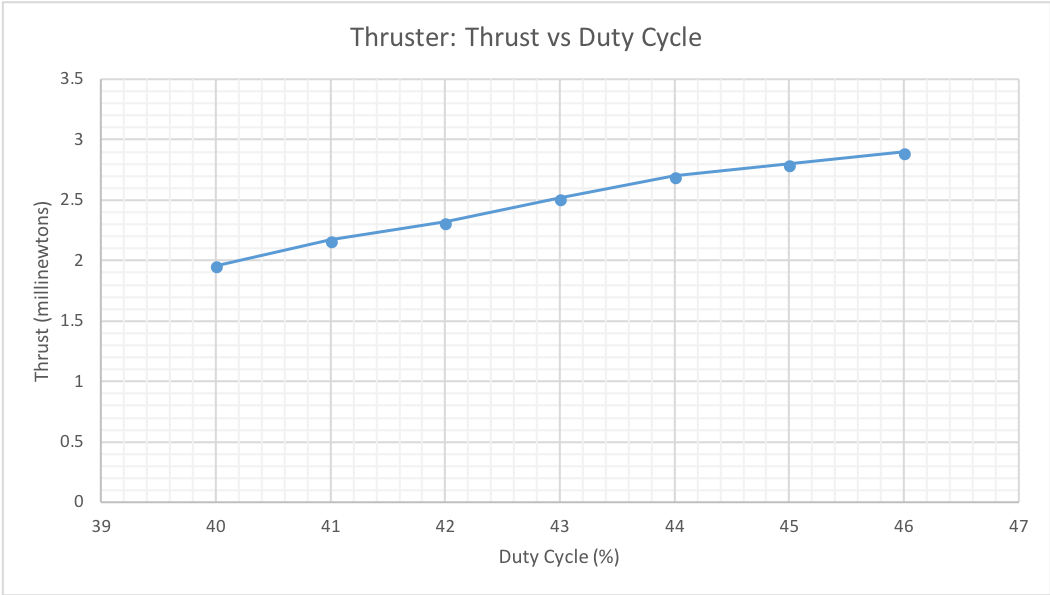
\includegraphics[width = 0.8\textwidth]{thruster_g2}
\caption{\label{fig:thruster_g2} Thrust versus duty cycle shows a linear relationship as expected.}
\end{figure}

\begin{figure}[h!]
\centering
\begin{subfigure}{0.49\textwidth}
\centering
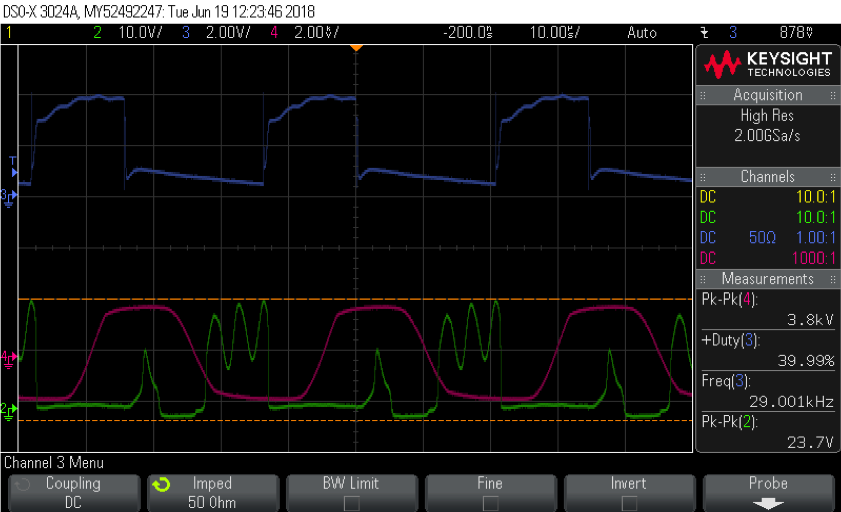
\includegraphics[width = \textwidth]{thruster_sc_21}
\caption{Duty cycle $=40\%$}
\label{fig:thruster_sc_21}
\end{subfigure}
\begin{subfigure}{0.49\textwidth}
\centering
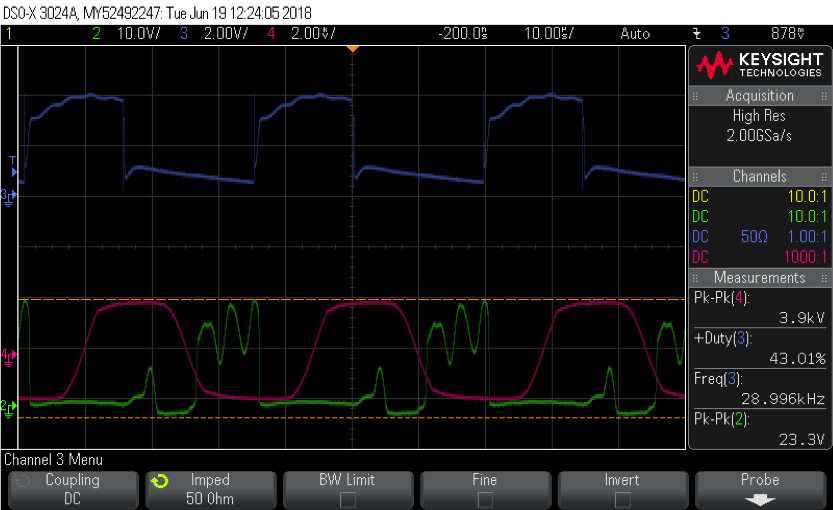
\includegraphics[width = \textwidth]{thruster_sc_23}
\caption{Duty cycle $=43\%$}
\label{fig:thruster_sc_23}
\end{subfigure}
\begin{subfigure}{0.49\textwidth}
\centering
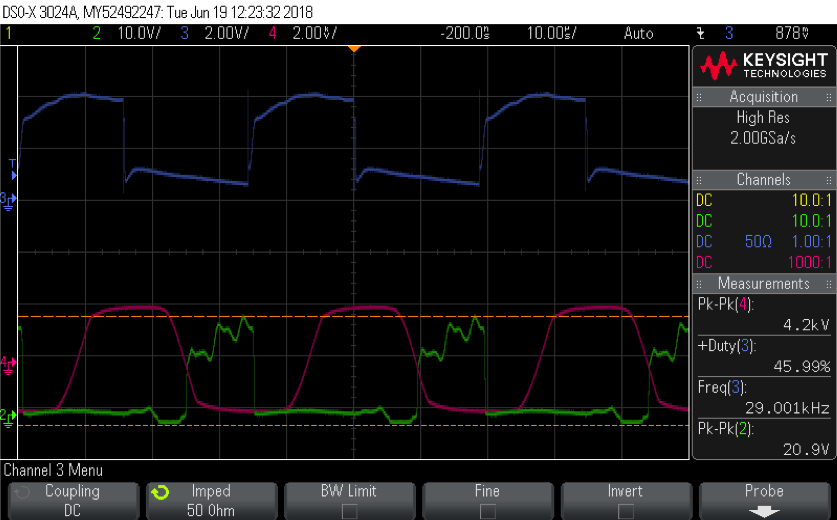
\includegraphics[width = \textwidth]{thruster_sc_22}
\caption{Duty cycle $=46\%$}
\label{fig:thruster_sc_22}
\end{subfigure}
\caption{\label{fig:thruster_duty} Scope reading showing the variation in driver voltage provided by the frequency generator, collector voltage, and transformer output for the thruster}
\end{figure}


\pagebreak
\subsubsection{Varying Input Frequency}

\begin{figure}[h!]
\centering
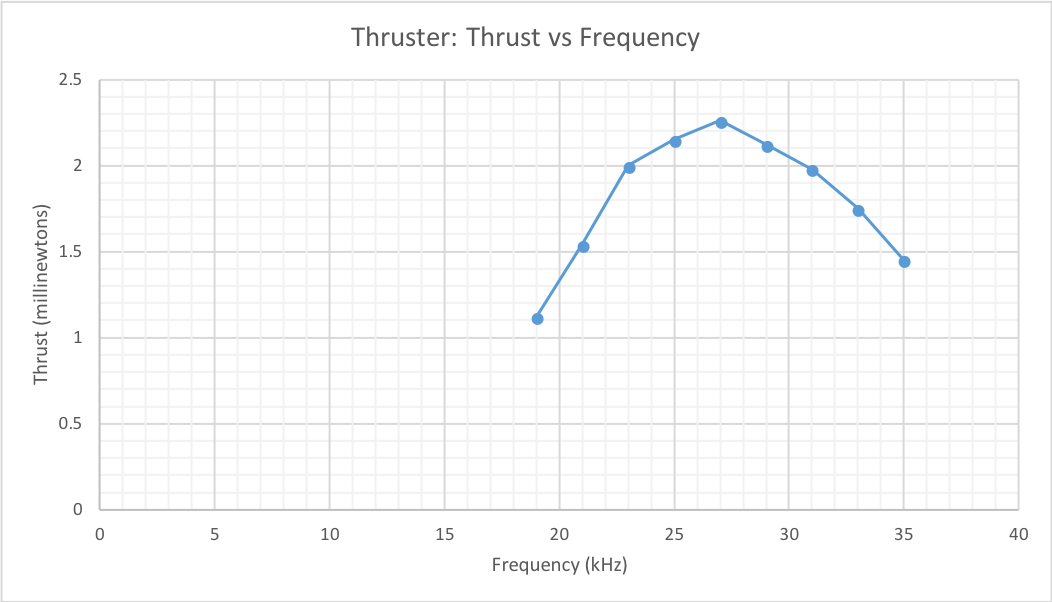
\includegraphics[width = 0.8\textwidth]{thruster_g3}
\caption{\label{fig:thruster_g3} Resonant behaviour is expected since the transformer is inductive and the voltage multiplier is capacitive. Thrust vs input frequency shows a resonant peak at 27 kHz.}
\end{figure}

\begin{figure}[h!]
\centering
\begin{subfigure}{0.47\textwidth}
\centering
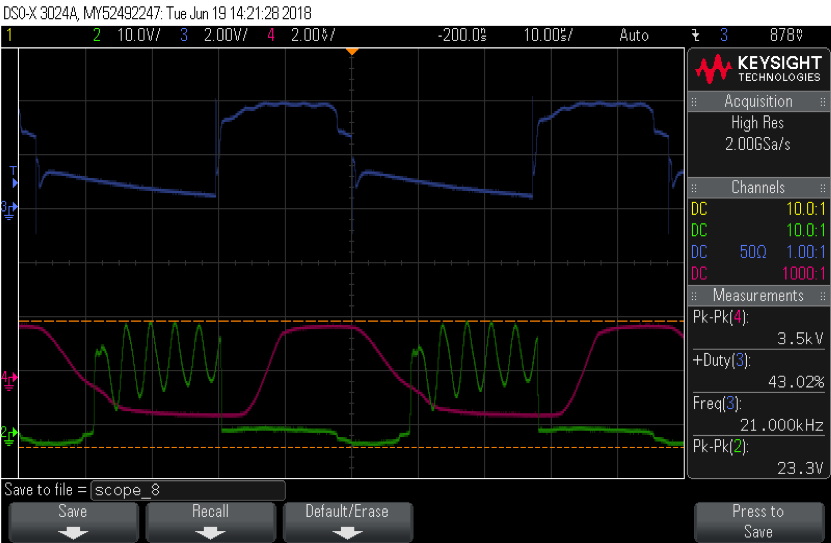
\includegraphics[width = \textwidth]{thruster_sc_31}
\caption{Frequency $= 21$ kHz}
\label{fig:thruster_sc_31}
\end{subfigure}
\begin{subfigure}{0.49\textwidth}
\centering
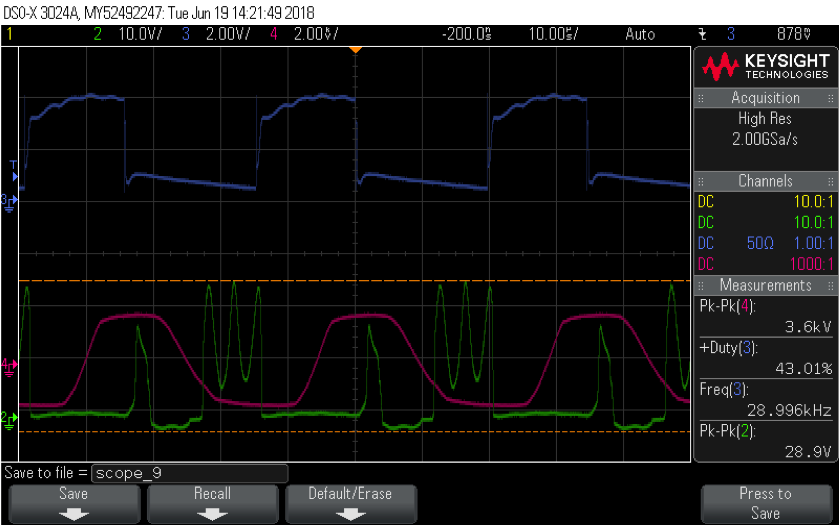
\includegraphics[width = \textwidth]{thruster_sc_33}
\caption{Frequency $= 29$ kHz}
\label{fig:thruster_sc_33}
\end{subfigure}
\begin{subfigure}{0.49\textwidth}
\centering
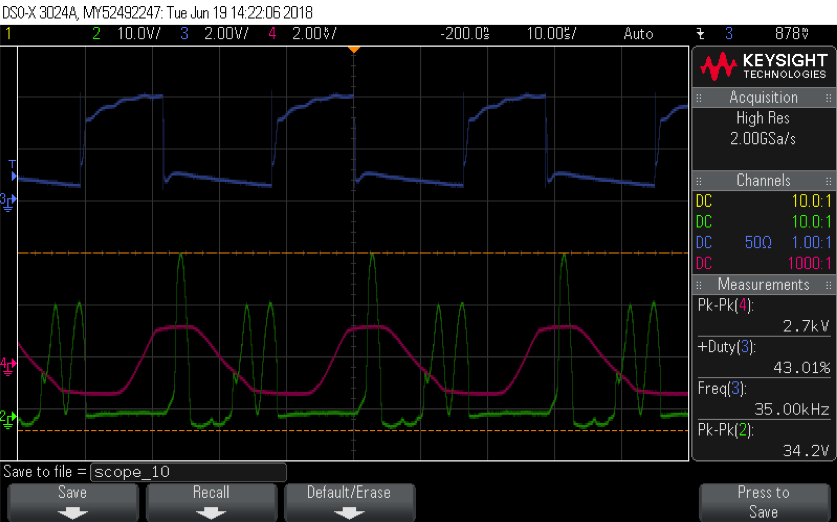
\includegraphics[width = \textwidth]{thruster_sc_32}
\caption{Frequency $= 35$ kHz}
\label{fig:thruster_sc_32}
\end{subfigure}
\caption{\label{fig:thruster_frequency} Scope reading showing the variation in driver voltage provided by the frequency generator, collector voltage, and transformer output for the thruster}
\end{figure}


\pagebreak
\subsubsection{Thrust vs Input Current}

\begin{figure}[h!]
\centering
\begin{subfigure}{0.49\textwidth}
\centering
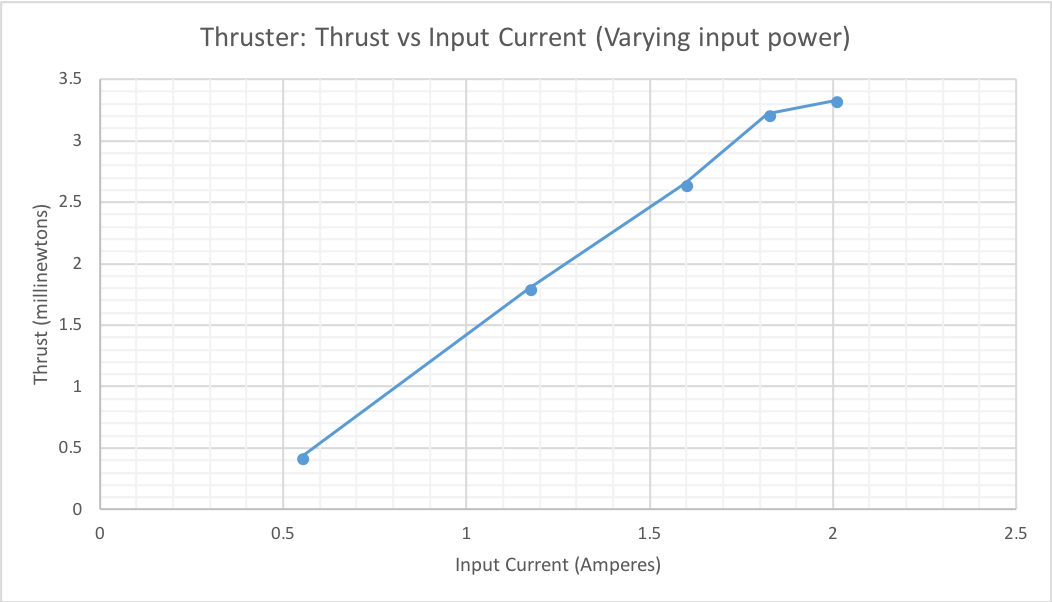
\includegraphics[width = \textwidth]{thruster_c1}
\caption{\label{fig:thruster_c1} Thrust versus input current while varying input power.}
\end{subfigure}
\begin{subfigure}{0.49\textwidth}
\centering
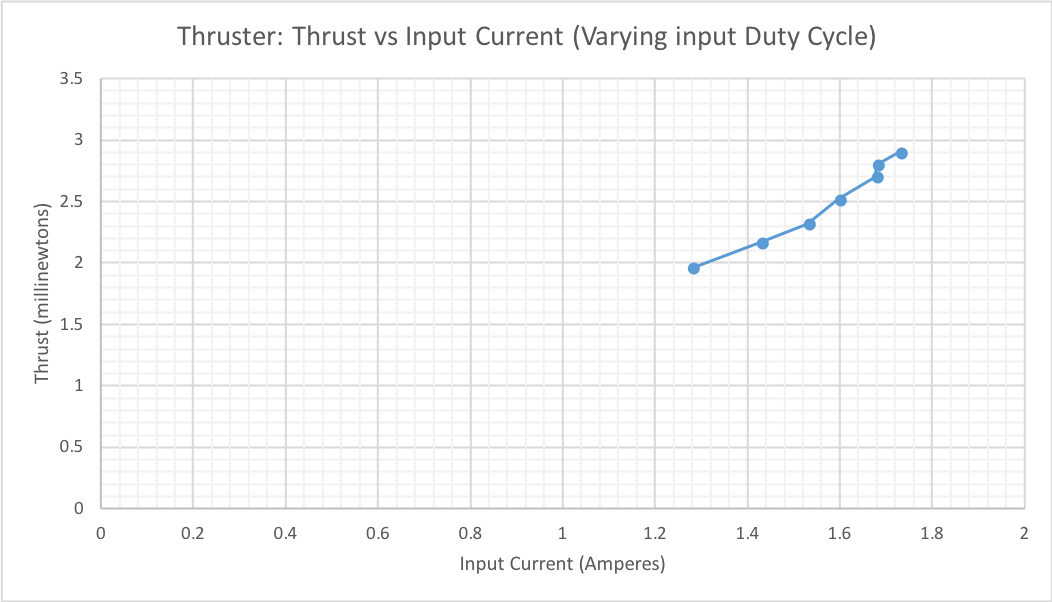
\includegraphics[width = \textwidth]{thruster_c2}
\caption{\label{fig:thruster_c2} Thrust versus input current while varying input duty cycle.}
\end{subfigure}
\begin{subfigure}{0.49\textwidth}
\centering
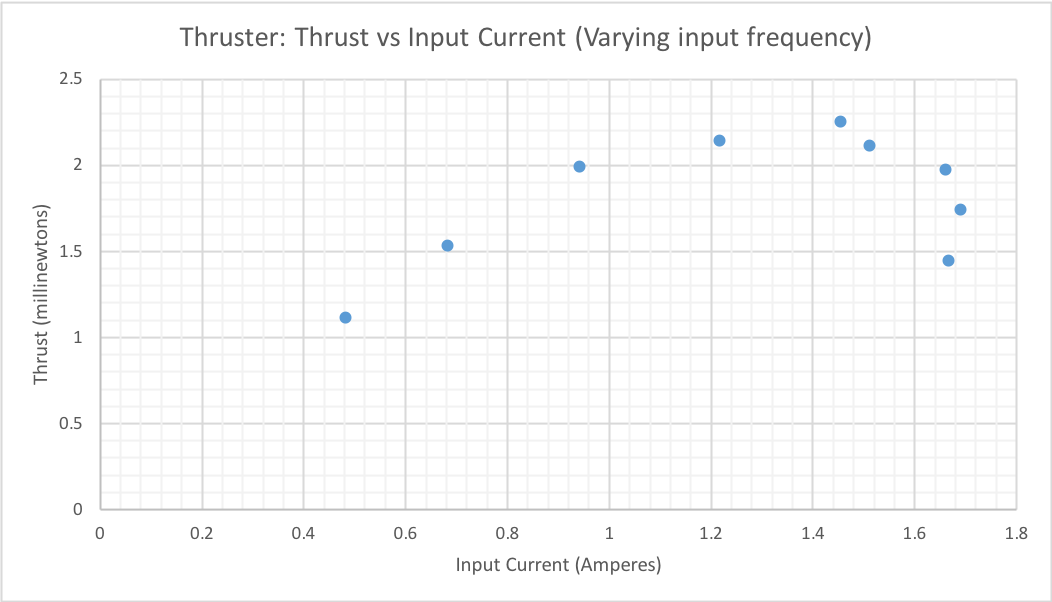
\includegraphics[width = \textwidth]{thruster_c3}
\caption{\label{fig:thruster_c3} Thrust versus input current while varying input frequency.}
\end{subfigure}
\caption{\label{fig:thruster_current} Variation of thrust with input current for the last three tests.}
\end{figure}

\subsubsection{Peak Thrust Frequency vs Duty Cycle}

\begin{figure}[h!]
\centering
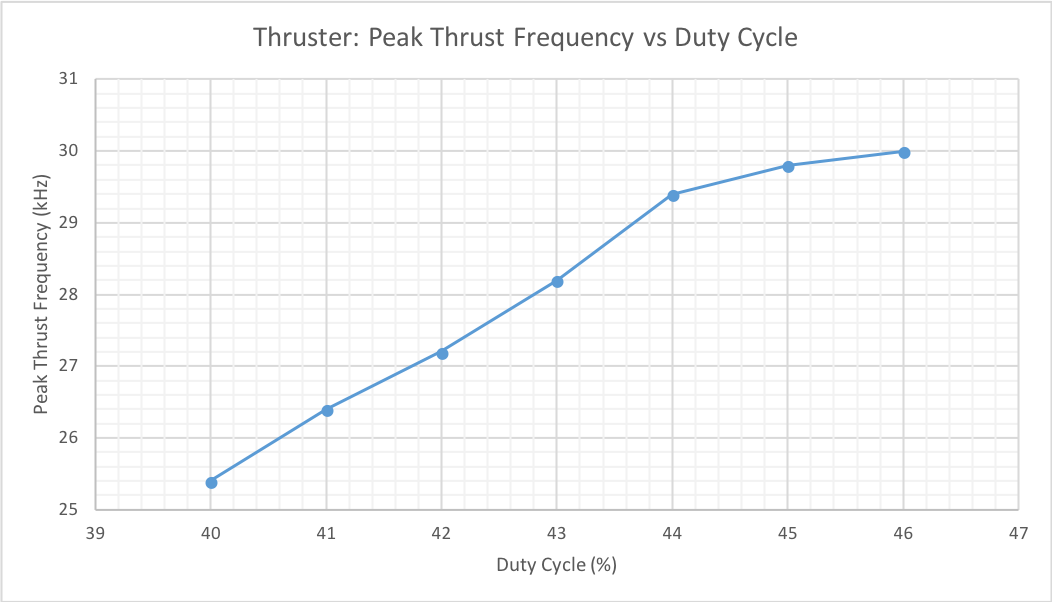
\includegraphics[width = 0.8\textwidth]{thruster_g4}
\caption{\label{fig:thruster_g4} Peak thrust frequency vs input duty cycle for the thruster.}
\end{figure}


\pagebreak
\subsection{The Ionocraft}


\subsubsection{Varying Input Power}

\begin{figure}[h!]
\centering
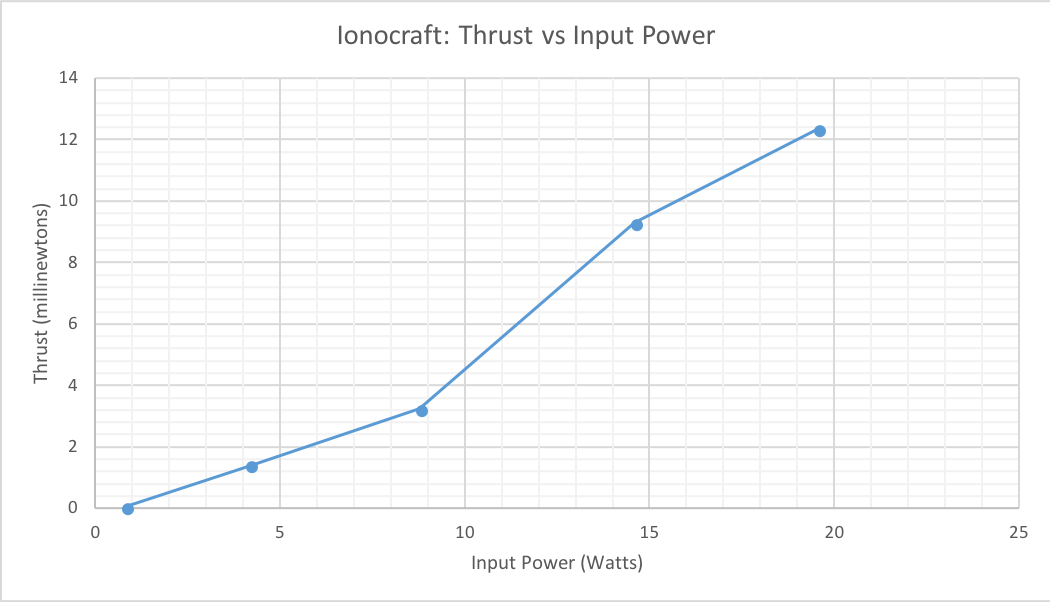
\includegraphics[width = 0.8\textwidth]{craft_g1}
\caption{\label{fig:craft_g1} Relationship between thrust and input power for the ionocraft}
\end{figure}

\begin{figure}[h!]
\centering
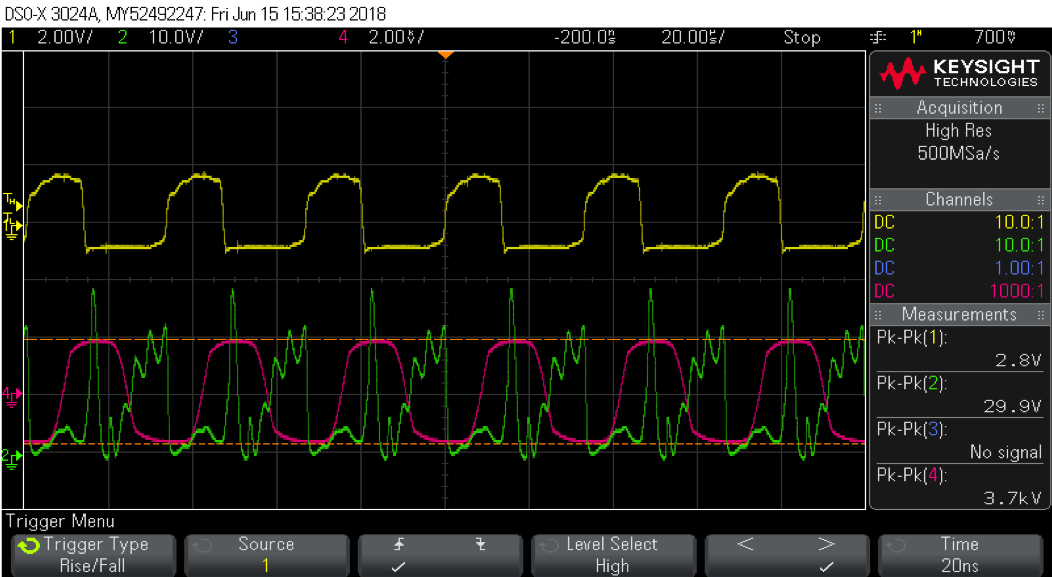
\includegraphics[width = 0.8\textwidth]{craft_sc_1}
\caption{\label{fig:craft_sc_1} Scope reading showing the driver voltage, collector voltage, and transformer output for the ionocraft}
\end{figure}

\pagebreak
\subsubsection{Varying Input Duty Cycle}

\begin{figure}[h!]
\centering
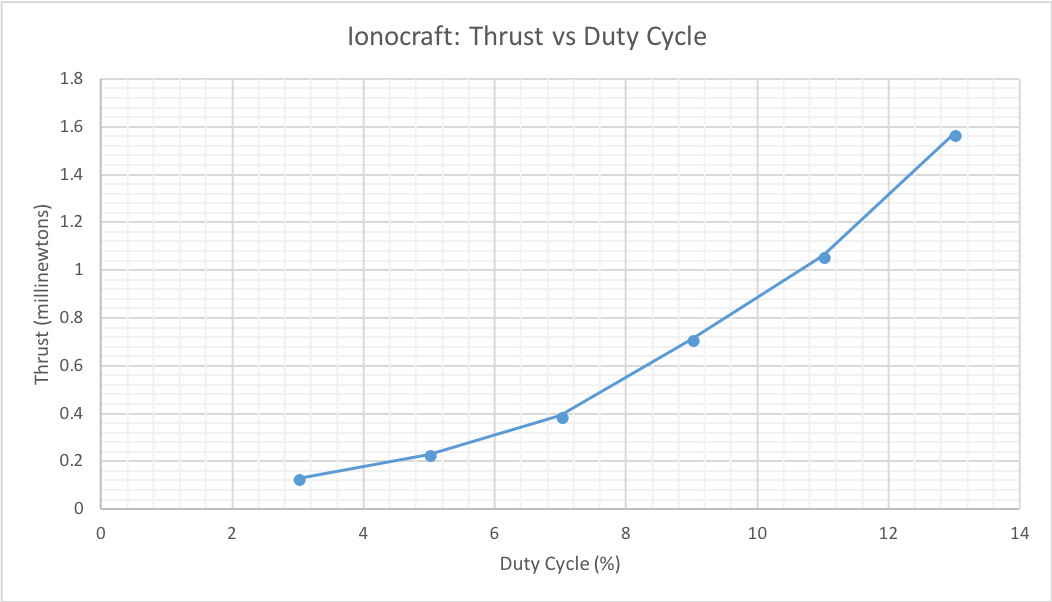
\includegraphics[width = 0.8\textwidth]{craft_g2}
\caption{\label{fig:craft_g2} Thrust versus input duty cycle at a constant input frequency of 26 kHz.}
\end{figure}

\begin{figure}[h!]
\centering
\begin{subfigure}{0.49\textwidth}
\centering
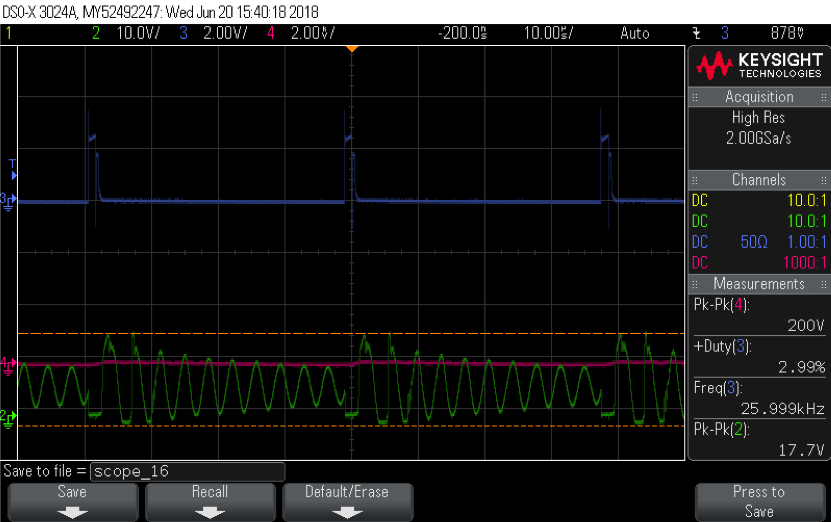
\includegraphics[width = \textwidth]{craft_sc_21}
\caption{Duty cycle $=3\%$}
\label{fig:craft_sc_21}
\end{subfigure}
\begin{subfigure}{0.49\textwidth}
\centering
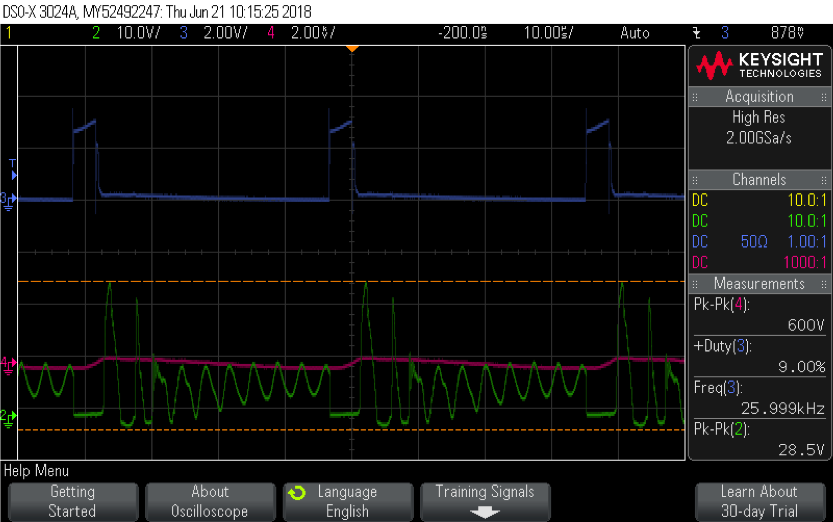
\includegraphics[width = \textwidth]{craft_sc_22}
\caption{Duty cycle $=9\%$}
\label{fig:craft_sc_22}
\end{subfigure}
\begin{subfigure}{0.49\textwidth}
\centering
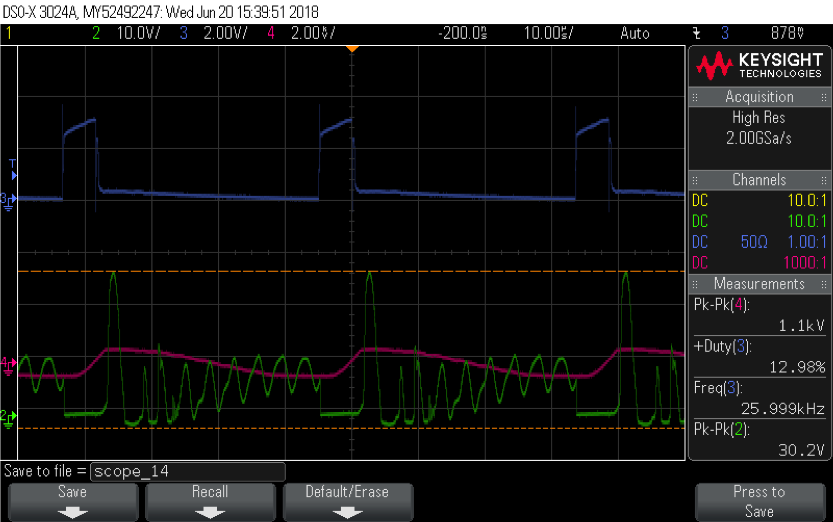
\includegraphics[width = \textwidth]{craft_sc_23}
\caption{Duty cycle $=13\%$}
\label{fig:craft_sc_23}
\end{subfigure}
\caption{\label{fig:thruster_duty} Scope reading showing the variation in driver voltage provided by the frequency generator, collector voltage, and transformer output for the ionocraft}
\end{figure}

\pagebreak
\subsubsection{Varying Input Frequency}

\begin{figure}[h!]
\centering
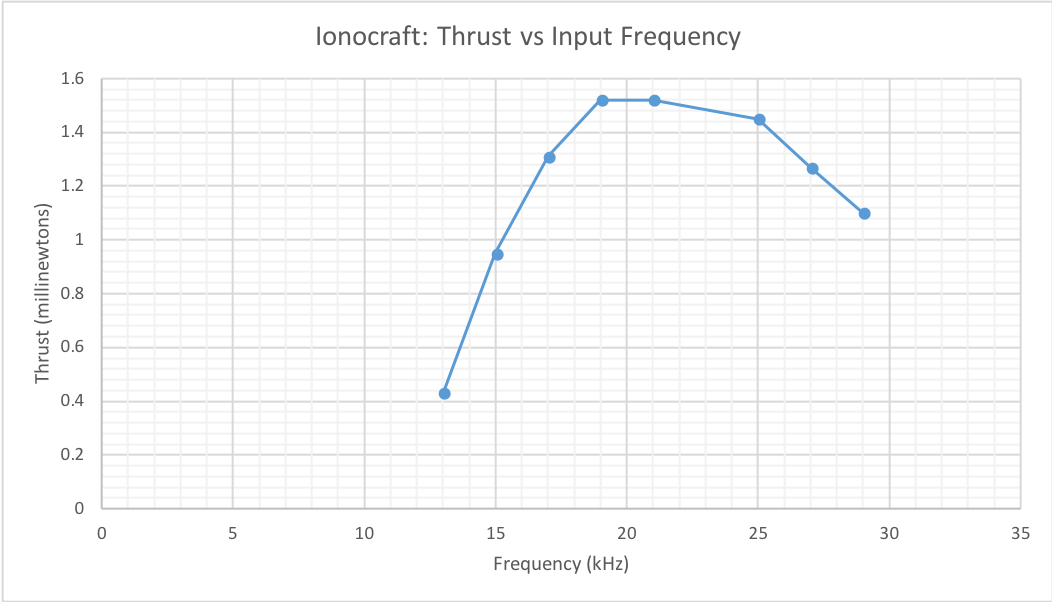
\includegraphics[width = 0.8\textwidth]{craft_g3}
\caption{\label{fig:craft_g3} Resonant behaviour is expected since the transformer is inductive and the voltage multiplier is capacitive. Thrust versus input frequency at a constant duty cycle of 21\% shows a resonant peak at 20 kHz.}
\end{figure}

\begin{figure}[h!]
\centering
\begin{subfigure}{0.49\textwidth}
\centering
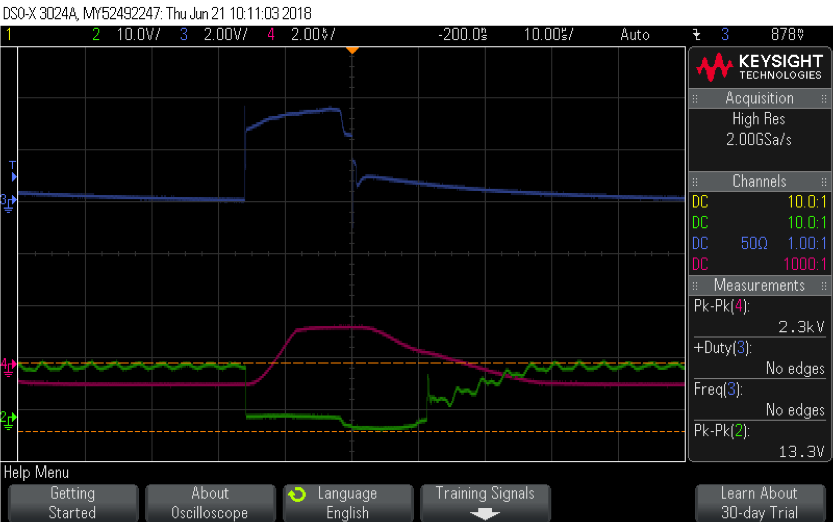
\includegraphics[width = \textwidth]{craft_sc_31}
\caption{Frequency $= 13$ kHz}
\label{fig:craft_sc_31}
\end{subfigure}
\begin{subfigure}{0.49\textwidth}
\centering
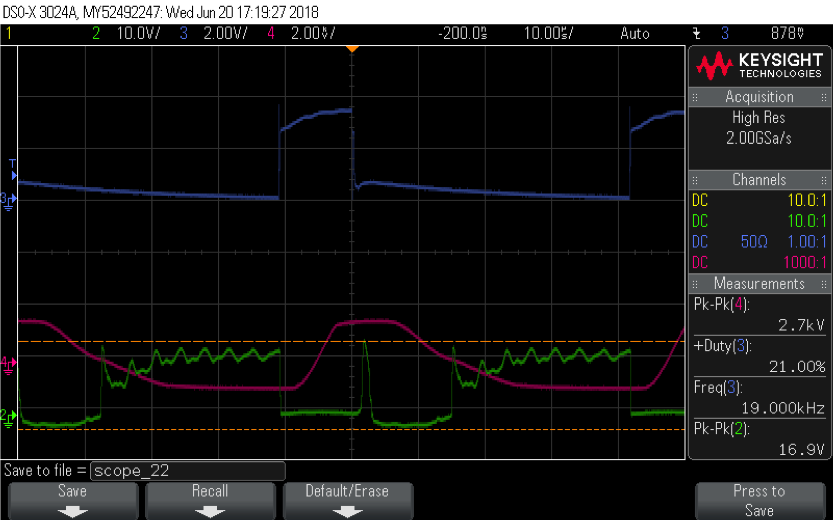
\includegraphics[width = \textwidth]{craft_sc_32}
\caption{Frequency $= 19$ kHz}
\label{fig:craft_sc_32}
\end{subfigure}
\begin{subfigure}{0.49\textwidth}
\centering
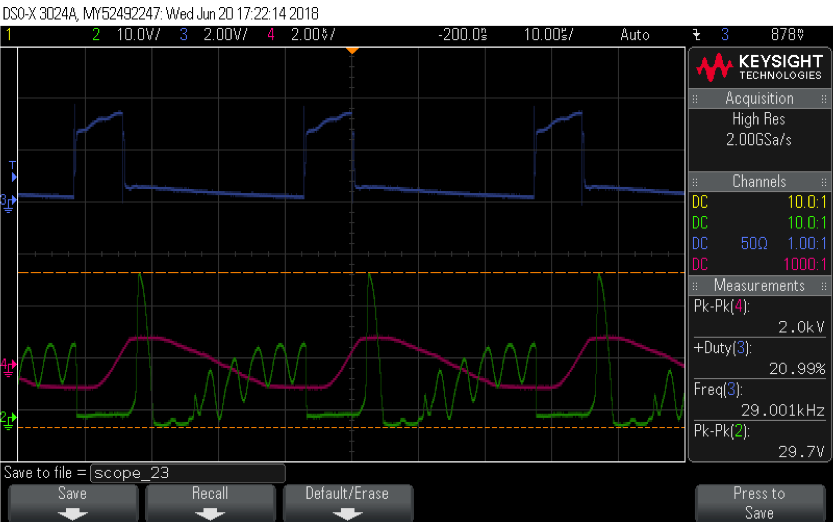
\includegraphics[width = \textwidth]{craft_sc_33}
\caption{Frequency $= 29$ kHz}
\label{fig:craft_sc_33}
\end{subfigure}
\caption{\label{fig:thruster_duty} Scope reading showing the variation in driver voltage provided by the frequency generator, collector voltage, and transformer output for the ionocraft}
\end{figure}

\pagebreak
\subsubsection{Thrust vs Input Current}

\begin{figure}[h!]
\centering
\begin{subfigure}{0.49\textwidth}
\centering
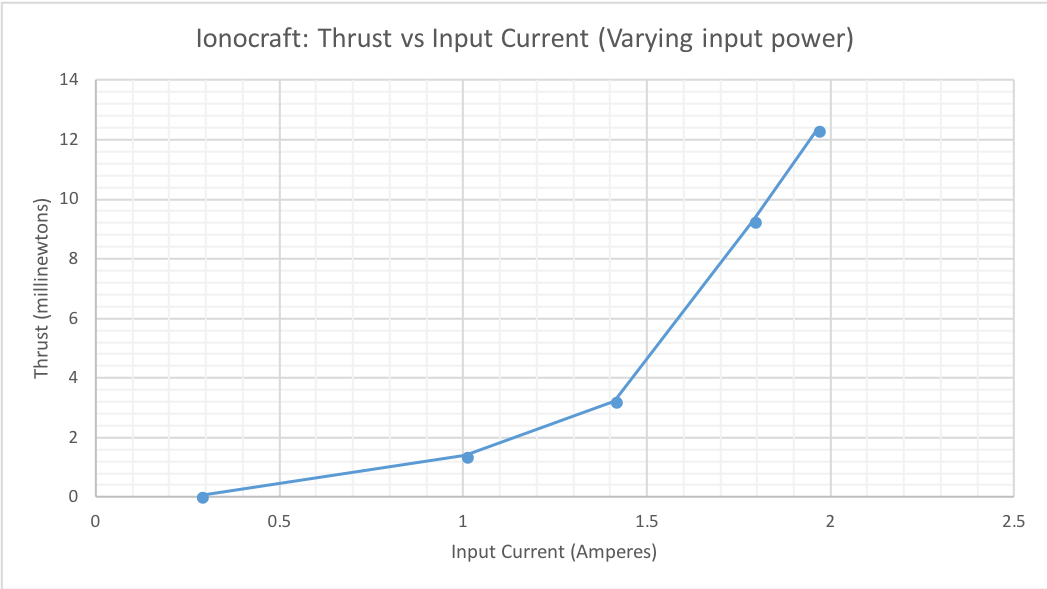
\includegraphics[width = \textwidth]{craft_c1}
\caption{\label{fig:craft_c1} Thrust versus input current while varying input power.}
\end{subfigure}
\begin{subfigure}{0.49\textwidth}
\centering
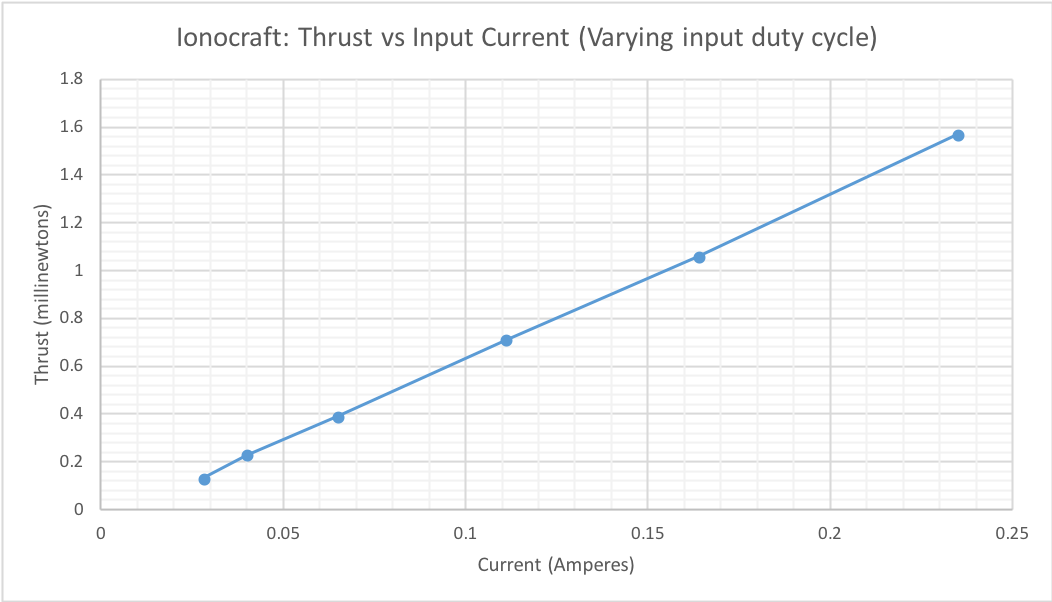
\includegraphics[width = \textwidth]{craft_c2}
\caption{\label{fig:craft_c2} Thrust versus input current while varying input duty cycle.}
\end{subfigure}
\begin{subfigure}{0.49\textwidth}
\centering
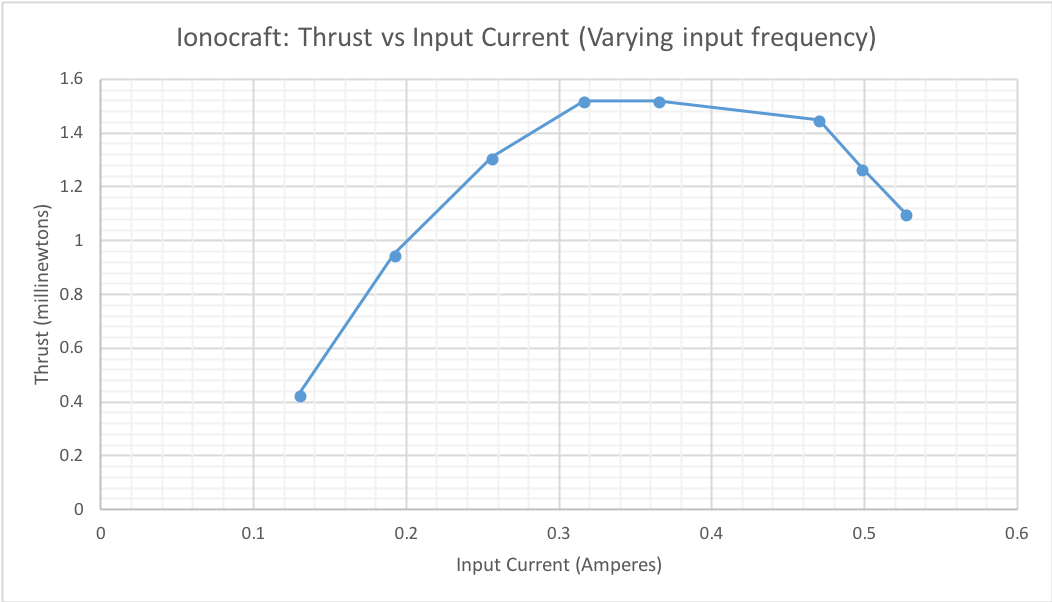
\includegraphics[width = \textwidth]{craft_c3}
\caption{\label{fig:craft_c3} Thrust versus input current while varying input frequency.}
\end{subfigure}
\caption{\label{fig:craft_current} Variation of thrust with input current for the last three tests.}
\end{figure}

\subsubsection{Peak Thrust Frequency vs Duty Cycle}

\begin{figure}[h!]
\centering
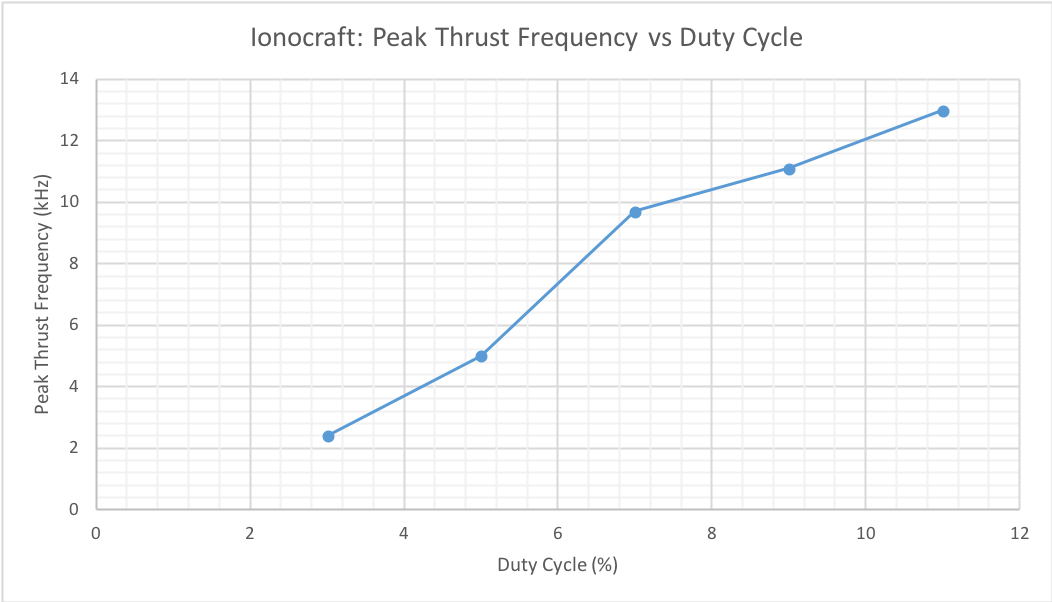
\includegraphics[width = 0.8\textwidth]{craft_g4}
\caption{\label{fig:craft_g4} Peak thrust frequency vs duty cycle for the ionocraft.}
\end{figure}

\subsubsection{Achieving liftoff with an HVDC Supply}

Since the 20 kV output was not enough to generate enough thrust to lift the ionocraft used for testing, brief access was gained to a Spellman SL150 HVDC power supply from the Wireless Power Lab in order to verify that the ionocraft works as intended. A risk assessment form was submitted to the department in order to ensure that the use of the supply would be directly supervised by a trained technician with prior experience in using HVDC power supplies.\\

A lighter craft was built using straws sliced in half as the skeleton of the craft, which reduced its weight from 1.64 grams to 1.1 grams. The vertical supports of the ionocraft were tethered by thread to prevent the craft from turning over and causing arcing. The craft began to achieve liftoff at 26 kV, 0.28 mA, and remained stable at a height of 4 cm (measured from the surface the the bottom of the vertical support) at 29 kV, 0.55mA.\\

The power supply was capable of supplying up to 40 kV, so more thrust could easily be generated while the craft was tethered to the same maximum height. However, increasing the length of the tethered thread beyond a height of 5 cm caused the craft to tumble due to the uneven thrust spread. Thus in order to increase the height achieved by the ionocraft, a stand would need to be fashioned to limit its movement to the Z direction.

\begin{figure}[h!]
\centering
\begin{subfigure}{0.49\textwidth}
\centering
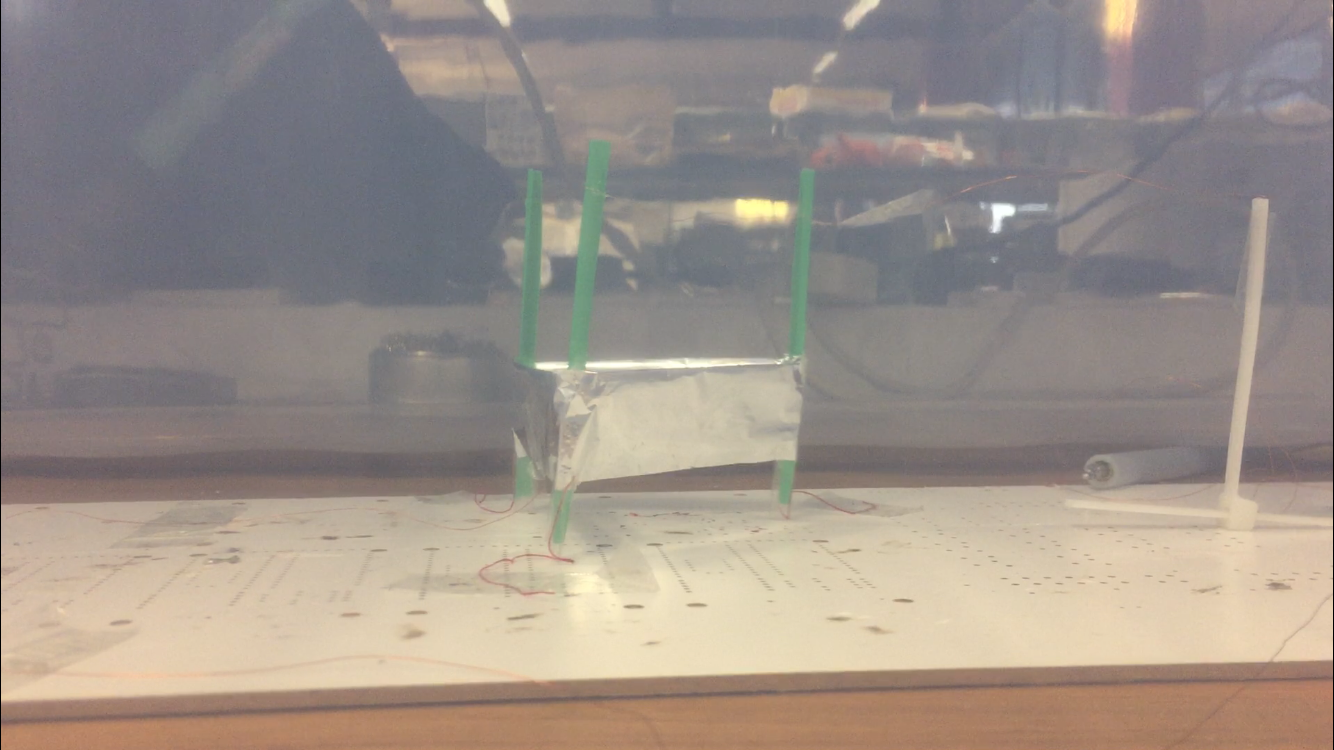
\includegraphics[width = \textwidth]{hvdc_1}
\caption{\label{fig:hvdc_1} }
\end{subfigure}
\begin{subfigure}{0.49\textwidth}
\centering
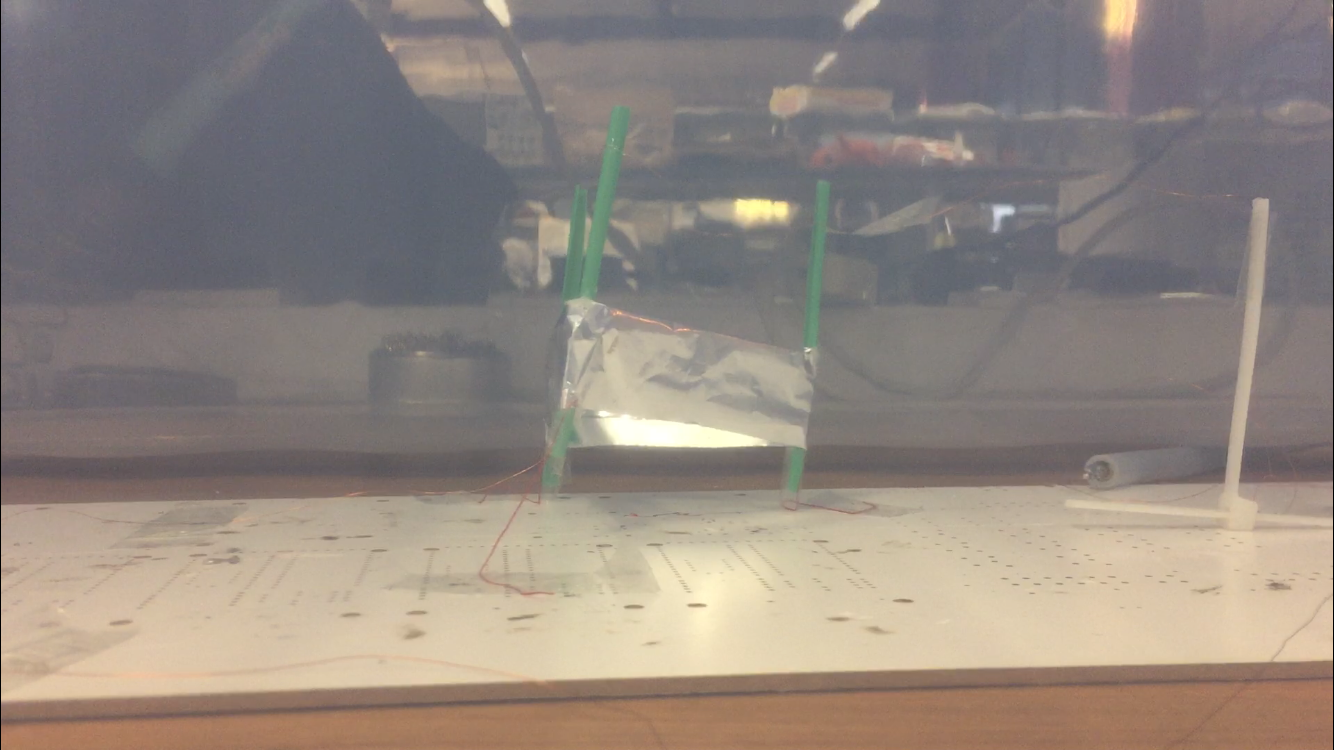
\includegraphics[width = \textwidth]{hvdc_2}
\caption{\label{fig:hvdc_2} }
\end{subfigure}
\begin{subfigure}{0.49\textwidth}
\centering
\includegraphics[width = \textwidth]{hvdc_3}
\caption{\label{fig:hvdc_3} }
\end{subfigure}
\caption{\label{fig:hvdc} Ionocraft achieves liftoff successfully with an HVDC power supply}
\end{figure}

\pagebreak
\section{Conclusions and Future Work}

Electric propulsion technology requires an incredibly large amount of voltage to produce very low thrust. Although the thrust output can be optimized incrementally by increasing the input power, increasing the duty cycle and operating at the resonant frequency of the system, the limiting factors are the magnitude of input voltage (required to accelerate the ions across the air gap) and the magnitude of current (for increased availability of ions). Until mankind invents a power source that has enough energy density to provide the magnitude of voltage and current required while being light enough fir liftoff, ion propulsion engines will remain impractical for use on Earth.\\

Future work for this project would include a more in depth investigation into the theory that would justify any design improvements and explain the  trends observed already. For example, a numerical analysis of the potential around the electrodes could give a more optimum positioning of the electrodes. A simple stand could be fabricated to restrict movement of the craft to the Z axis without any pitch, roll, yaw or drift in the X or Y direction. Multiple stage ionocrafts could be built with multiple electrodes releasing ions for improving thrust output. A PID controller could then be implemented to control the thrust output in order to maintain the craft at a certain height. An investigation into high density, low weight power sources might even lead to a design for an autonomous micro-thruster.


\pagebreak

\begin{thebibliography}{9}

\bibitem{nasa}
Advanced Space Transportation Technology Summary: Electric Propulsion Available at: https://www.nasa.gov/centers/marshall/pdf/100403main\_electric\_propulsion.pdf [Accessed 6 May 2018].

\bibitem{space}
Space.com. (2018). Ion Thruster Prototype Breaks Records in Tests, Could Send Humans to Mars. [online] Available at: https://www.space.com/38444-mars-thruster-design-breaks-records.html [Accessed 4 May 2018].

\bibitem{comstat}
Lev, D., Emsellem, G. and Hallock, A. (2017). The Rise of the Electric Age for Satellite Propulsion. New Space, 5(1), pp.4-14.

\bibitem{goebel} 
Goebel, D. and Katz, I. (2008). Fundamentals of electric propulsion. Hoboken, N.J.: Wiley, pp.1-10.

\bibitem{ionthruster}
Unconventional Rocket Drives - Ion Drives (2018). [online]\\
Available at: http://www2.ee.ic.ac.uk/derek.low08/yr2proj/ion.htm [Accessed 1 May 2018].

\bibitem{ehdperform}
Masuyama, K. and Barrett, S. (2013). On the performance of electrohydrodynamic propulsion. Proceedings of the Royal Society A: Mathematical, Physical and Engineering Sciences, 469(2154), pp.20120623-20120623.

\bibitem{mit}
Szondy, D. (2018). MIT researchers study electro-hydrodynamic thrust. [online] Newatlas.com. Available at: https://newatlas.com/mit-ionocraft/26908/ [Accessed 2 May 2018].

\bibitem{verge}
The Verge. (2018). Ionic thrusters could power the ultra-efficient, stealth drones of the future. [online] Available at: https://www.theverge.com/2013/4/3/4178708/ionic-thrusters-more-efficient-than-jet-engines-says-MIT-study [Accessed 3 May 2018].

\bibitem{park}
Large.stanford.edu. (2018). Ionocraft: Electrohydrodynamic Ion-Propelled Aircraft. [online] Available at: http://large.stanford.edu/courses/2017/ph240/park1/ [Accessed 5 May 2018].

\bibitem{femm}
Femm.info. (2018). Finite Element Method Magnetics: HomePage. [online] Available at: http://www.femm.info/wiki/HomePage [Accessed 4 Jun. 2018].

\bibitem{prototype}
Reifsnyder, A. (2018). Build an Ionic Thruster like NASA Uses for Space Propulsion | Make:. [online] Make: DIY Projects and Ideas for Makers. Available at: https://makezine.com/projects/ionic-thruster/ [Accessed 6 May 2018].

\bibitem{plasmaball}
Amazon.co.uk. (2018). Global Gizmos 8-inch Magic Plasma Ball. [online] Available at: https://www.amazon.co.uk/dp/B009RQLI36/ref=pe\_1909131\_77697121\_tnp\_email\_TE\_AMZLdp\_1 [Accessed 6 Jun. 2018].

\bibitem{panicker}
Panicker, P. (2003). Ionisation of air by corona discharge. [online] Arc.uta.edu. Available at: http:\/\/arc.uta.edu\/publications\/td\_files\/paniker.pdf [Accessed 21 Jun. 2018].

\bibitem{workshop}
WorkshopScience. (n.d.). Ionocraft Project. [online] Available at: https:\/\/workshopscience.com\/ionocraft-project\/ [Accessed 21 Jun. 2018].

\end{thebibliography}

\end{document}
